\documentclass[11pt]{article}
\usepackage[margin=0.95in]{geometry}
\usepackage{lmodern}
\usepackage[T1]{fontenc}
\usepackage{microtype}
\usepackage{xcolor}
\usepackage{amsmath,amssymb,mathtools}
\usepackage{booktabs,tabularx,longtable,array,multirow}
\newcolumntype{Y}{>{\raggedright\arraybackslash}X}
\usepackage{enumitem}
\usepackage{caption}
\usepackage{listings}
\usepackage{tikz}
\usetikzlibrary{arrows.meta,positioning,shapes.geometric,calc}
\usepackage[hidelinks]{hyperref}

\definecolor{navy}{HTML}{1B3A4B}
\definecolor{teal}{HTML}{0E6B66}
\definecolor{tealfaint}{HTML}{E5F3F1}
\definecolor{gold}{HTML}{A56B10}
\definecolor{goldfaint}{HTML}{FBF3E0}
\definecolor{brick}{HTML}{8E3A3A}
\definecolor{brickfaint}{HTML}{F8E8E6}
\definecolor{leaf}{HTML}{2F6F4E}
\definecolor{leaffaint}{HTML}{E5F2EA}
\definecolor{slate}{HTML}{5E6A75}
\definecolor{linec}{HTML}{243140}
\definecolor{paper}{HTML}{F7F4EF}
\definecolor{unk}{HTML}{E4E1DA}
\definecolor{freec}{HTML}{F7F7F5}
\definecolor{occ}{HTML}{2C333A}
\definecolor{enc}{HTML}{C45C4A}
\definecolor{frcell}{HTML}{2A9D8F}
\definecolor{codebg}{HTML}{F4F1EA}

\lstset{
  basicstyle=\ttfamily\footnotesize,
  backgroundcolor=\color{codebg},
  frame=single,
  rulecolor=\color{linec},
  breaklines=true,
  columns=fullflexible,
  keepspaces=true,
  xleftmargin=1em,
  framexleftmargin=0.6em
}

\setlist[itemize]{leftmargin=1.2em, itemsep=0.2em, topsep=0.35em}
\setlist[enumerate]{leftmargin=1.4em, itemsep=0.25em, topsep=0.35em}
\captionsetup{font=small, labelfont=bf, skip=6pt}
\setlength{\parskip}{0.35em}
\setlength{\parindent}{1.15em}
\setlength{\emergencystretch}{2em}
\renewcommand{\arraystretch}{1.15}

\newcommand{\code}[1]{\texttt{#1}}
\newcommand{\commit}[1]{\texttt{#1}}

% Shared technical figures. Each command emits a tikzpicture only.
% Captions and labels live in the manuscripts so the two papers can differ.

\newcommand{\FigArchitecture}{%
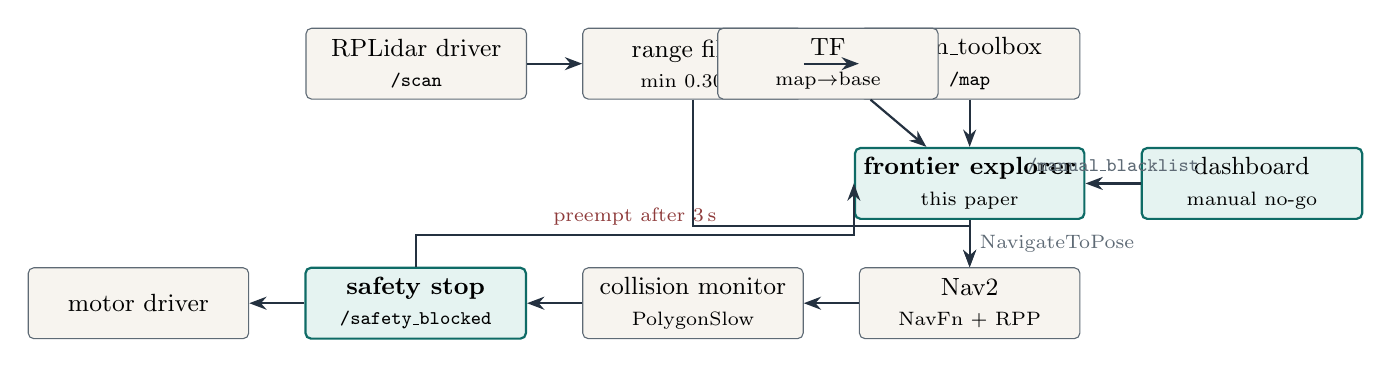
\begin{tikzpicture}[
  font=\small,
  node distance=6mm and 7mm,
  box/.style={draw=linec, rounded corners=2pt, align=center, fill=white,
              minimum width=28mm, minimum height=9mm, inner sep=3pt},
  custom/.style={box, fill=tealfaint, draw=teal, thick},
  oss/.style={box, fill=paper, draw=slate},
  arr/.style={-{Stealth[length=2.2mm]}, draw=linec, thick}
]
  \node[oss] (lidar) {RPLidar driver\\{\scriptsize\texttt{/scan}}};
  \node[oss, right=of lidar] (filter) {range filter\\{\scriptsize min 0.30\,m}};
  \node[oss, right=of filter] (slam) {slam\_toolbox\\{\scriptsize\texttt{/map}}};
  \node[custom, below=of slam] (expl) {\textbf{frontier explorer}\\{\scriptsize this paper}};
  \node[oss, below=of expl] (nav) {Nav2\\{\scriptsize NavFn + RPP}};
  \node[oss, left=of nav] (coll) {collision monitor\\{\scriptsize PolygonSlow}};
  \node[custom, left=of coll] (safe) {\textbf{safety stop}\\{\scriptsize\texttt{/safety\_blocked}}};
  \node[oss, left=of safe] (drv) {motor driver};
  \node[oss, above=of expl, xshift=-18mm] (tf) {TF\\{\scriptsize map$\rightarrow$base}};
  \node[custom, right=of expl] (dash) {dashboard\\{\scriptsize manual no-go}};

  \draw[arr] (lidar) -- (filter);
  \draw[arr] (filter) -- (slam);
  \draw[arr] (slam) -- (expl);
  \draw[arr] (expl) -- node[right, font=\scriptsize, text=slate] {NavigateToPose} (nav);
  \draw[arr] (nav) -- (coll);
  \draw[arr] (coll) -- (safe);
  \draw[arr] (safe) -- (drv);
  \draw[arr] (tf) -- (expl);
  \draw[arr] (dash) -- node[above, font=\scriptsize, text=slate] {\texttt{/manual\_blacklist}} (expl);
  \draw[arr] (safe.north) -- ++(0,4mm) -| node[pos=0.25, above, font=\scriptsize, text=brick] {preempt after 3\,s} (expl.west);
  \draw[arr] (filter.south) -- ++(0,-16mm) -| (nav.north);
\end{tikzpicture}%
}

\newcommand{\FigCommandChain}{%
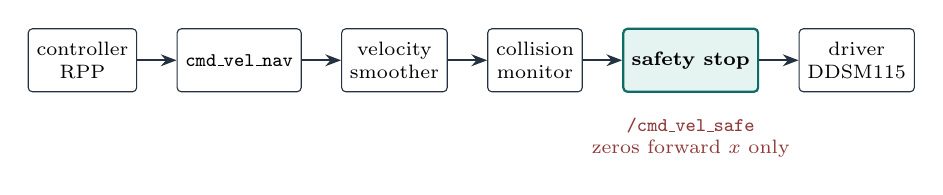
\begin{tikzpicture}[
  font=\scriptsize,
  arr/.style={-{Stealth[length=2mm]}, draw=linec, thick},
  n/.style={draw=linec, rounded corners=1.5pt, align=center, fill=white,
            inner sep=3pt, minimum height=8mm},
  c/.style={n, fill=tealfaint, draw=teal, thick}
]
  \node[n] (a) {controller\\RPP};
  \node[n, right=5mm of a] (b) {\texttt{cmd\_vel\_nav}};
  \node[n, right=5mm of b] (c) {velocity\\smoother};
  \node[n, right=5mm of c] (d) {collision\\monitor};
  \node[c, right=5mm of d] (e) {\textbf{safety stop}};
  \node[n, right=5mm of e] (f) {driver\\DDSM115};
  \draw[arr] (a) -- (b);
  \draw[arr] (b) -- (c);
  \draw[arr] (c) -- (d);
  \draw[arr] (d) -- (e);
  \draw[arr] (e) -- (f);
  \node[below=2mm of e, align=center, text=brick, font=\scriptsize]
    {\texttt{/cmd\_vel\_safe}\\zeros forward $x$ only};
\end{tikzpicture}%
}

\newcommand{\FigPipeline}{%
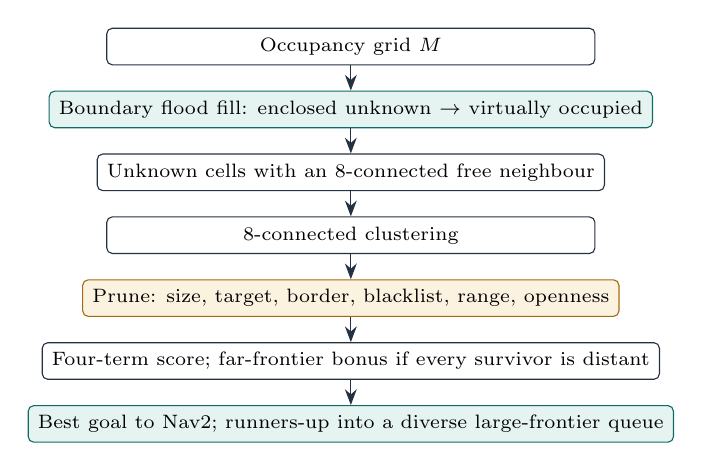
\begin{tikzpicture}[
  font=\scriptsize,
  node distance=3.2mm,
  s/.style={draw=linec, rounded corners=2pt, align=center, fill=white,
            minimum width=62mm, inner sep=3.5pt},
  d/.style={s, fill=goldfaint, draw=gold},
  k/.style={s, fill=tealfaint, draw=teal},
  arr/.style={-{Stealth[length=2mm]}, draw=linec}
]
  \node[s] (m) {Occupancy grid $M$};
  \node[k, below=of m] (e) {Boundary flood fill: enclosed unknown $\rightarrow$ virtually occupied};
  \node[s, below=of e] (f) {Unknown cells with an 8-connected free neighbour};
  \node[s, below=of f] (c) {8-connected clustering};
  \node[d, below=of c] (p) {Prune: size, target, border, blacklist, range, openness};
  \node[s, below=of p] (sc) {Four-term score; far-frontier bonus if every survivor is distant};
  \node[k, below=of sc] (q) {Best goal to Nav2; runners-up into a diverse large-frontier queue};
  \draw[arr] (m) -- (e);
  \draw[arr] (e) -- (f);
  \draw[arr] (f) -- (c);
  \draw[arr] (c) -- (p);
  \draw[arr] (p) -- (sc);
  \draw[arr] (sc) -- (q);
\end{tikzpicture}%
}

\newcommand{\FigEnclosed}{%
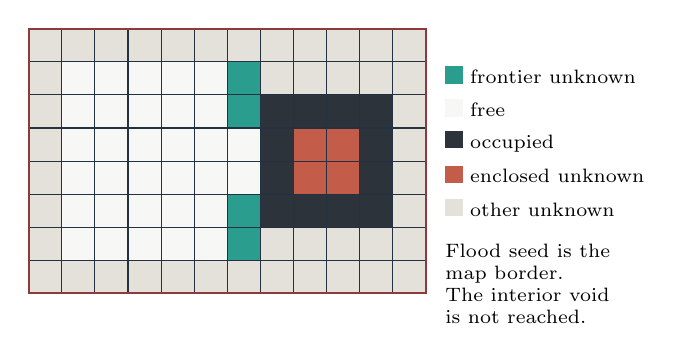
\begin{tikzpicture}[scale=0.42, font=\scriptsize]
  \foreach \x in {0,...,11} {
    \foreach \y in {0,...,7} {
      \fill[unk] (\x,\y) rectangle ++(1,1);
    }
  }
  % reachable free corridor and room
  \foreach \x/\y in {1/1,2/1,3/1,4/1,5/1,1/2,2/2,3/2,4/2,5/2,1/3,2/3,3/3,4/3,5/3,6/3,1/4,2/4,3/4,4/4,5/4,6/4,1/5,2/5,3/5,4/5,5/5,1/6,2/6,3/6,4/6,5/6} {
    \fill[freec] (\x,\y) rectangle ++(1,1);
  }
  % obstacle shell
  \foreach \x/\y in {7/2,8/2,9/2,10/2,7/3,10/3,7/4,10/4,7/5,8/5,9/5,10/5} {
    \fill[occ] (\x,\y) rectangle ++(1,1);
  }
  % enclosed unknown inside the shell
  \foreach \x/\y in {8/3,9/3,8/4,9/4} {
    \fill[enc] (\x,\y) rectangle ++(1,1);
  }
  % frontier-like unknown touching free on the right of the room
  \foreach \x/\y in {6/1,6/2,6/5,6/6} {
    \fill[frcell] (\x,\y) rectangle ++(1,1);
  }
  \draw[linec, thin] (0,0) grid (12,8);
  \draw[brick, thick] (0,0) rectangle (12,8);
  \node[anchor=west, font=\scriptsize] at (12.3,6.6) {\textcolor{frcell}{\rule{2.2mm}{2.2mm}} frontier unknown};
  \node[anchor=west, font=\scriptsize] at (12.3,5.6) {\textcolor{freec}{\rule{2.2mm}{2.2mm}} free};
  \node[anchor=west, font=\scriptsize] at (12.3,4.6) {\textcolor{occ}{\rule{2.2mm}{2.2mm}} occupied};
  \node[anchor=west, font=\scriptsize] at (12.3,3.6) {\textcolor{enc}{\rule{2.2mm}{2.2mm}} enclosed unknown};
  \node[anchor=west, font=\scriptsize] at (12.3,2.6) {\textcolor{unk}{\rule{2.2mm}{2.2mm}} other unknown};
  \node[align=left, anchor=north west, font=\scriptsize] at (12.3,1.8)
    {Flood seed is the\\map border.\\The interior void\\is not reached.};
\end{tikzpicture}%
}

\newcommand{\FigPrune}{%
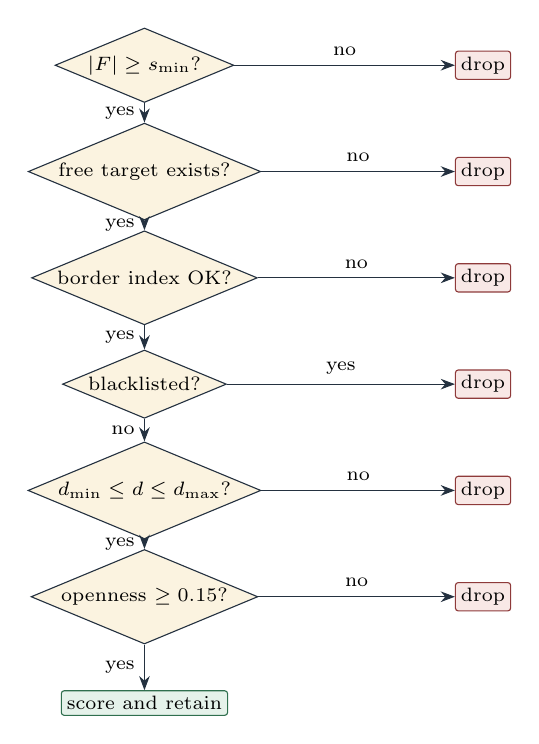
\begin{tikzpicture}[
  font=\scriptsize,
  dec/.style={draw=linec, diamond, aspect=2.4, align=center, inner sep=1pt, fill=goldfaint},
  rej/.style={draw=brick, fill=brickfaint, rounded corners=1pt, align=center, inner sep=2pt},
  ok/.style={draw=leaf, fill=leaffaint, rounded corners=1pt, align=center, inner sep=2pt},
  arr/.style={-{Stealth[length=1.8mm]}, draw=linec}
]
  \node[dec] (s) at (0,0) {$|F|\ge s_{\min}$?};
  \node[rej] (r1) at (4.3,0) {drop};
  \node[dec] (t) at (0,-1.35) {free target exists?};
  \node[rej] (r2) at (4.3,-1.35) {drop};
  \node[dec] (b) at (0,-2.7) {border index OK?};
  \node[rej] (r3) at (4.3,-2.7) {drop};
  \node[dec] (k) at (0,-4.05) {blacklisted?};
  \node[rej] (r4) at (4.3,-4.05) {drop};
  \node[dec] (d) at (0,-5.4) {$d_{\min}\le d\le d_{\max}$?};
  \node[rej] (r5) at (4.3,-5.4) {drop};
  \node[dec] (o) at (0,-6.75) {openness $\ge 0.15$?};
  \node[rej] (r6) at (4.3,-6.75) {drop};
  \node[ok] (g) at (0,-8.1) {score and retain};
  \draw[arr] (s) -- node[left] {yes} (t);
  \draw[arr] (s) -- node[above] {no} (r1);
  \draw[arr] (t) -- node[left] {yes} (b);
  \draw[arr] (t) -- node[above] {no} (r2);
  \draw[arr] (b) -- node[left] {yes} (k);
  \draw[arr] (b) -- node[above] {no} (r3);
  \draw[arr] (k) -- node[left] {no} (d);
  \draw[arr] (k) -- node[above] {yes} (r4);
  \draw[arr] (d) -- node[left] {yes} (o);
  \draw[arr] (d) -- node[above] {no} (r5);
  \draw[arr] (o) -- node[left] {yes} (g);
  \draw[arr] (o) -- node[above] {no} (r6);
\end{tikzpicture}%
}

\newcommand{\FigScore}{%
\begin{tikzpicture}[x=1.15cm, y=0.55cm, font=\scriptsize]
  \draw[linec] (0,0) -- (0,5.2);
  \draw[linec] (0,2.6) -- (8.6,2.6);
  \node[rotate=90, anchor=south] at (-0.45,2.6) {contribution};
  % zero line at y=2.6; scale 4 units per 1.0 score
  \foreach \y/\lab in {0.6/-0.5, 2.6/0, 4.6/+0.5} {
    \draw[slate] (-0.08,\y) -- (0.08,\y);
  }
  \node[left] at (0,0.6) {$-0.5$};
  \node[left] at (0,2.6) {$0$};
  \node[left] at (0,4.6) {$+0.5$};
  % A contributions: +0.90, -0.40, -0.25, +0.42  but bars relative to zero
  % clip display: size +0.90 is off scale if 4 per unit... use 2.2 per unit
  % redo: unit = 2.2 cm per 1.0, zero at 0
  % I'll draw from scratch with y unit already set. Let me use absolute.
\end{tikzpicture}%
}

% The placeholder above is replaced by a real waterfall. Defined separately.
\renewcommand{\FigScore}{%
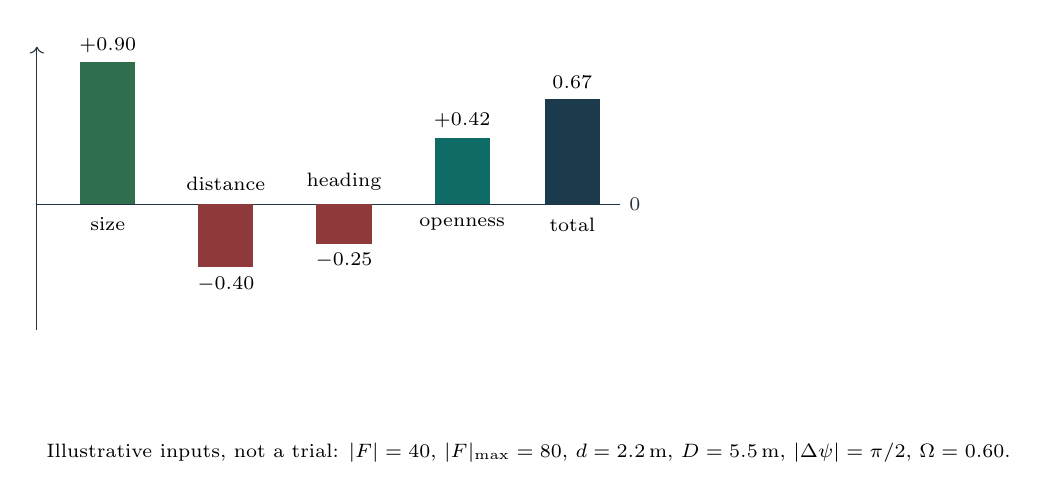
\begin{tikzpicture}[font=\scriptsize]
  \def\z{0}
  % bars: size +0.90, dist -0.40, head -0.25, open +0.42, total 0.67
  \draw[->, linec] (0,0) -- (0,3.6) node[above] {};
  \draw[linec] (0,1.6) -- (7.4,1.6) node[right] {$0$};
  \begin{scope}[shift={(0.55,1.6)}]
    \fill[leaf] (0,0) rectangle (0.7,1.80);
    \node[above] at (0.35,1.80) {$+0.90$};
    \node[below] at (0.35,-0.05) {size};
  \end{scope}
  \begin{scope}[shift={(2.05,1.6)}]
    \fill[brick] (0,-0.80) rectangle (0.7,0);
    \node[below] at (0.35,-0.80) {$-0.40$};
    \node[above] at (0.35,0.05) {distance};
  \end{scope}
  \begin{scope}[shift={(3.55,1.6)}]
    \fill[brick] (0,-0.50) rectangle (0.7,0);
    \node[below] at (0.35,-0.50) {$-0.25$};
    \node[above] at (0.35,0.05) {heading};
  \end{scope}
  \begin{scope}[shift={(5.05,1.6)}]
    \fill[teal] (0,0) rectangle (0.7,0.84);
    \node[above] at (0.35,0.84) {$+0.42$};
    \node[below] at (0.35,-0.05) {openness};
  \end{scope}
  \begin{scope}[shift={(6.45,1.6)}]
    \fill[navy] (0,0) rectangle (0.7,1.34);
    \node[above] at (0.35,1.34) {$0.67$};
    \node[below] at (0.35,-0.05) {total};
  \end{scope}
  \node[anchor=west, align=left, font=\scriptsize] at (0,-1.55)
    {Illustrative inputs, not a trial: $|F|=40$, $|F|_{\max}=80$, $d=2.2$\,m, $D=5.5$\,m, $|\Delta\psi|=\pi/2$, $\Omega=0.60$.};
\end{tikzpicture}%
}

\newcommand{\FigLifecycle}{%
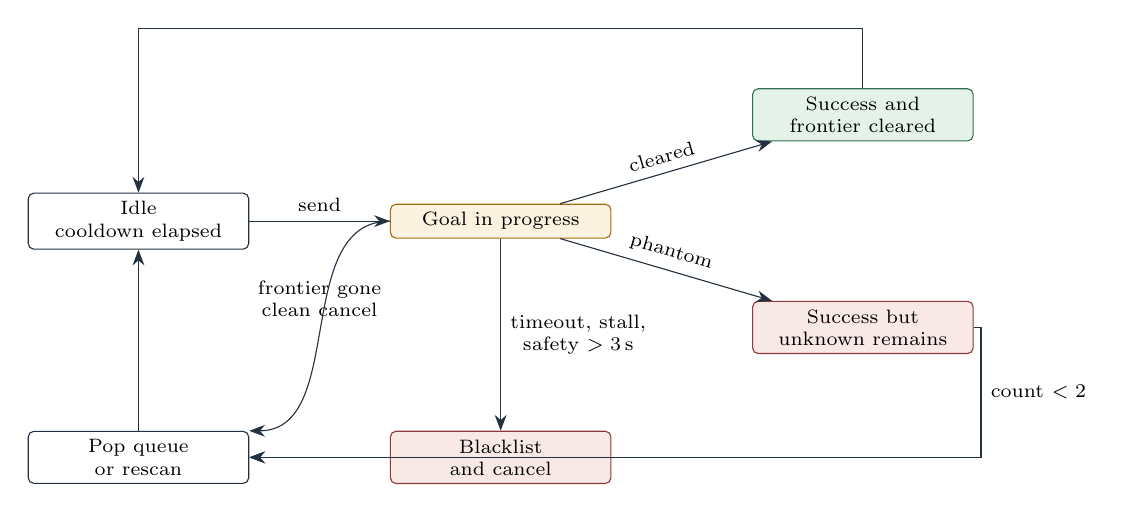
\begin{tikzpicture}[
  font=\scriptsize,
  st/.style={draw=linec, rounded corners=2pt, align=center, fill=white,
             minimum width=28mm, inner sep=3pt},
  hot/.style={st, fill=goldfaint, draw=gold},
  bad/.style={st, fill=brickfaint, draw=brick},
  good/.style={st, fill=leaffaint, draw=leaf},
  arr/.style={-{Stealth[length=2mm]}, draw=linec}
]
  \node[st] (idle) at (0,0) {Idle\\cooldown elapsed};
  \node[hot] (nav) at (4.6,0) {Goal in progress};
  \node[good] (ok) at (9.2,1.35) {Success and\\frontier cleared};
  \node[bad] (ph) at (9.2,-1.35) {Success but\\unknown remains};
  \node[bad] (bl) at (4.6,-3.0) {Blacklist\\and cancel};
  \node[st] (sw) at (0,-3.0) {Pop queue\\or rescan};
  \draw[arr] (idle) -- node[above] {send} (nav);
  \draw[arr] (nav) -- node[above, sloped] {cleared} (ok);
  \draw[arr] (nav) -- node[above, sloped] {phantom} (ph);
  \draw[arr] (ok) -- ++(0,1.1) -| (idle);
  \draw[arr] (ph) -- ++(1.5,0) |- node[pos=0.25, right] {count $<2$} (sw);
  \draw[arr] (nav) -- node[right, align=center] {timeout, stall,\\safety $>3$\,s} (bl);
  \draw[arr] (nav.west) to[out=180, in=0] node[above, align=center] {frontier gone\\clean cancel} (sw.north east);
  \draw[arr] (bl) -- (sw);
  \draw[arr] (sw) -- (idle);
\end{tikzpicture}%
}

\newcommand{\FigRecovery}{%
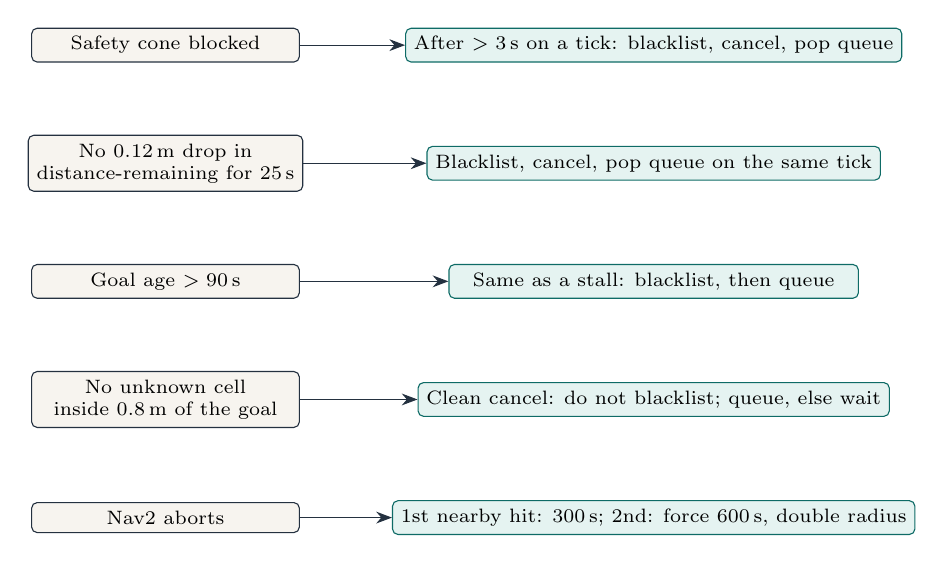
\begin{tikzpicture}[
  font=\scriptsize,
  ev/.style={draw=linec, rounded corners=2pt, align=center, fill=paper,
             minimum width=34mm, inner sep=3pt},
  act/.style={draw=teal, rounded corners=2pt, align=center, fill=tealfaint,
              minimum width=52mm, inner sep=3pt},
  arr/.style={-{Stealth[length=2mm]}, draw=linec}
]
  \node[ev] (a) at (0,0) {Safety cone blocked};
  \node[act] (a2) at (6.2,0) {After $>3$\,s on a tick: blacklist, cancel, pop queue};
  \node[ev] (b) at (0,-1.5) {No $0.12$\,m drop in\\distance-remaining for $25$\,s};
  \node[act] (b2) at (6.2,-1.5) {Blacklist, cancel, pop queue on the same tick};
  \node[ev] (c) at (0,-3.0) {Goal age $>90$\,s};
  \node[act] (c2) at (6.2,-3.0) {Same as a stall: blacklist, then queue};
  \node[ev] (d) at (0,-4.5) {No unknown cell\\inside $0.8$\,m of the goal};
  \node[act] (d2) at (6.2,-4.5) {Clean cancel: do not blacklist; queue, else wait};
  \node[ev] (e) at (0,-6.0) {Nav2 aborts};
  \node[act] (e2) at (6.2,-6.0) {1st nearby hit: $300$\,s; 2nd: force $600$\,s, double radius};
  \draw[arr] (a) -- (a2);
  \draw[arr] (b) -- (b2);
  \draw[arr] (c) -- (c2);
  \draw[arr] (d) -- (d2);
  \draw[arr] (e) -- (e2);
\end{tikzpicture}%
}

\newcommand{\FigQueue}{%
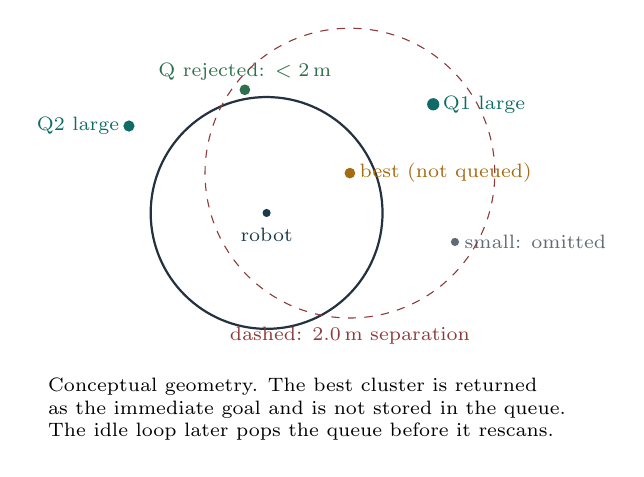
\begin{tikzpicture}[scale=0.92, font=\scriptsize]
  \draw[linec, thick] (0,0) circle (1.6);
  \fill[navy] (0,0) circle (1.6pt) node[below=2pt] {robot};
  \fill[gold] (1.15,0.55) circle (2.1pt) node[right] {best (not queued)};
  \fill[leaf] (-0.3,1.7) circle (2.1pt) node[above] {Q rejected: $<2$\,m};
  \fill[teal] (2.3,1.5) circle (2.4pt) node[right] {Q1 large};
  \fill[teal] (-1.9,1.2) circle (2.2pt) node[left] {Q2 large};
  \fill[slate] (2.6,-0.4) circle (1.6pt) node[right] {small: omitted};
  \draw[brick, dashed] (1.15,0.55) circle (2.0);
  \node[brick] at (1.15,-1.7) {dashed: $2.0$\,m separation};
  \node[align=left, anchor=north west] at (-3.15,-2.15)
    {Conceptual geometry. The best cluster is returned\\
     as the immediate goal and is not stored in the queue.\\
     The idle loop later pops the queue before it rescans.};
\end{tikzpicture}%
}

\newcommand{\FigRelax}{%
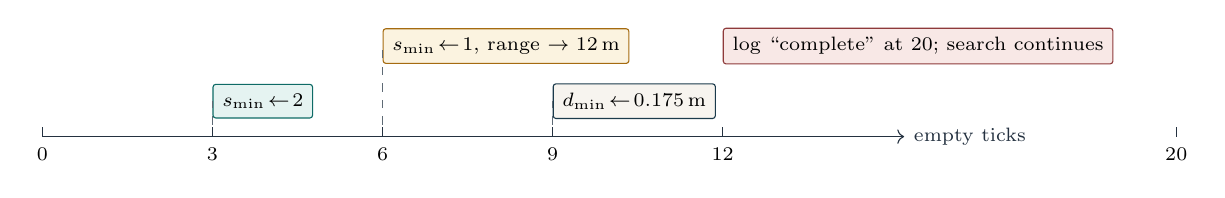
\begin{tikzpicture}[font=\scriptsize, x=0.72cm]
  \draw[->, linec] (0,0) -- (15.2,0) node[right] {empty ticks};
  \foreach \t in {0,3,6,9,12,20} {
    \draw[linec] (\t,0) -- (\t,0.12);
    \node[below] at (\t,-0.02) {\t};
  }
  \node[draw=teal, fill=tealfaint, rounded corners=1pt, anchor=west] at (3,0.45) {$s_{\min}\!\leftarrow\!2$};
  \node[draw=gold, fill=goldfaint, rounded corners=1pt, anchor=west] at (6,1.15) {$s_{\min}\!\leftarrow\!1$, range $\rightarrow 12$\,m};
  \node[draw=navy, fill=paper, rounded corners=1pt, anchor=west] at (9,0.45) {$d_{\min}\!\leftarrow\!0.175$\,m};
  \node[draw=brick, fill=brickfaint, rounded corners=1pt, anchor=west] at (12,1.15) {log ``complete'' at 20; search continues};
  \draw[slate, dashed] (3,0.15) -- (3,0.45);
  \draw[slate, dashed] (6,0.15) -- (6,1.15);
  \draw[slate, dashed] (9,0.15) -- (9,0.45);
\end{tikzpicture}%
}

\newcommand{\FigTimeline}{%
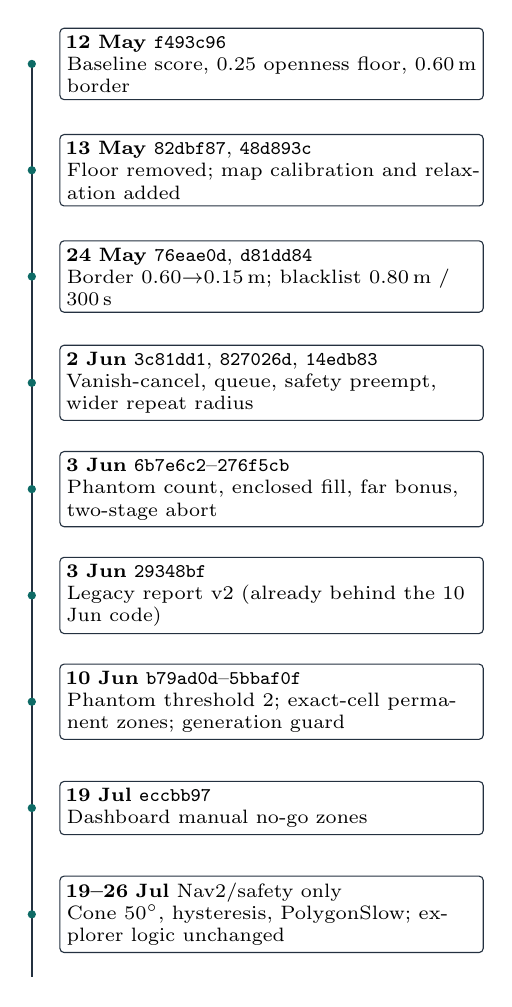
\begin{tikzpicture}[
  font=\scriptsize,
  ev/.style={draw=linec, fill=white, rounded corners=1.5pt, align=left,
             inner sep=2.5pt, text width=52mm},
  arr/.style={draw=linec, thick}
]
  \draw[arr] (0,0) -- (0,-11.6);
  \foreach \y in {0,-1.35,-2.7,-4.05,-5.4,-6.75,-8.1,-9.45,-10.8} {
    \fill[teal] (0,\y) circle (1.5pt);
  }
  \node[ev, anchor=west] at (0.35,0) {\textbf{12 May} \texttt{f493c96}\\Baseline score, 0.25 openness floor, 0.60\,m border};
  \node[ev, anchor=west] at (0.35,-1.35) {\textbf{13 May} \texttt{82dbf87}, \texttt{48d893c}\\Floor removed; map calibration and relaxation added};
  \node[ev, anchor=west] at (0.35,-2.7) {\textbf{24 May} \texttt{76eae0d}, \texttt{d81dd84}\\Border 0.60$\rightarrow$0.15\,m; blacklist 0.80\,m / 300\,s};
  \node[ev, anchor=west] at (0.35,-4.05) {\textbf{2 Jun} \texttt{3c81dd1}, \texttt{827026d}, \texttt{14edb83}\\Vanish-cancel, queue, safety preempt, wider repeat radius};
  \node[ev, anchor=west] at (0.35,-5.4) {\textbf{3 Jun} \texttt{6b7e6c2}--\texttt{276f5cb}\\Phantom count, enclosed fill, far bonus, two-stage abort};
  \node[ev, anchor=west] at (0.35,-6.75) {\textbf{3 Jun} \texttt{29348bf}\\Legacy report v2 (already behind the 10 Jun code)};
  \node[ev, anchor=west] at (0.35,-8.1) {\textbf{10 Jun} \texttt{b79ad0d}--\texttt{5bbaf0f}\\Phantom threshold 2; exact-cell permanent zones; generation guard};
  \node[ev, anchor=west] at (0.35,-9.45) {\textbf{19 Jul} \texttt{eccbb97}\\Dashboard manual no-go zones};
  \node[ev, anchor=west] at (0.35,-10.8) {\textbf{19--26 Jul} Nav2/safety only\\Cone $50^\circ$, hysteresis, PolygonSlow; explorer logic unchanged};
\end{tikzpicture}%
}

\newcommand{\FigScaleBug}{%
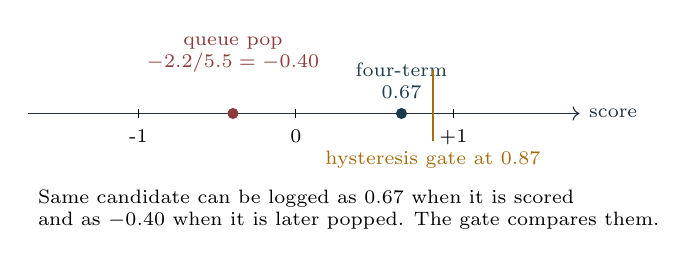
\begin{tikzpicture}[font=\scriptsize]
  \draw[->, linec] (-3.4,0) -- (3.6,0) node[right] {score};
  \foreach \x/\lab in {-2/-1, 0/0, 2/+1} {
    \draw (\x,-0.06) -- (\x,0.06);
    \node[below] at (\x,-0.08) {\lab};
  }
  \fill[navy] (1.34,0) circle (2pt) node[above=2pt, align=center] {four-term\\$0.67$};
  \fill[brick] (-0.8,0) circle (2pt) node[above=4mm, align=center, text=brick] {queue pop\\$-2.2/5.5=-0.40$};
  \draw[gold, thick] (1.74,-0.35) -- (1.74,0.55);
  \node[gold, below] at (1.74,-0.35) {hysteresis gate at $0.87$};
  \node[align=left, anchor=north west] at (-3.4,-0.85)
    {Same candidate can be logged as $0.67$ when it is scored\\
     and as $-0.40$ when it is later popped. The gate compares them.};
\end{tikzpicture}%
}

\newcommand{\FigSafetyCone}{%
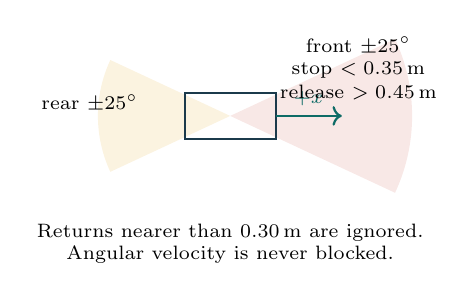
\begin{tikzpicture}[scale=1.05, font=\scriptsize]
  \fill[brickfaint] (0,0) -- (25:2.2) arc (25:-25:2.2) -- cycle;
  \fill[goldfaint] (0,0) -- (155:1.6) arc (155:205:1.6) -- cycle;
  \draw[navy, thick] (-0.55,-0.28) rectangle (0.55,0.28);
  \draw[->, teal, thick] (0.55,0) -- (1.35,0) node[midway, above] {$+x$};
  \node at (1.55,0.85) {front $\pm 25^\circ$};
  \node at (1.55,0.55) {stop $<0.35$\,m};
  \node at (1.55,0.28) {release $>0.45$\,m};
  \node at (-1.7,0.15) {rear $\pm 25^\circ$};
  \node[align=center] at (0,-1.55) {Returns nearer than $0.30$\,m are ignored.\\Angular velocity is never blocked.};
\end{tikzpicture}%
}

\newcommand{\FigExperiment}{%
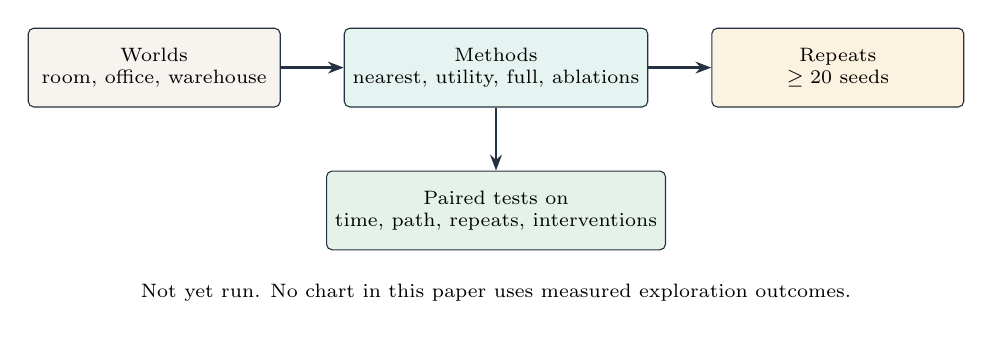
\begin{tikzpicture}[
  font=\scriptsize,
  b/.style={draw=linec, rounded corners=2pt, align=center, fill=white,
            minimum width=32mm, minimum height=10mm, inner sep=3pt},
  arr/.style={-{Stealth[length=2mm]}, draw=linec, thick}
]
  \node[b, fill=paper] (w) {Worlds\\room, office, warehouse};
  \node[b, fill=tealfaint, right=8mm of w] (m) {Methods\\nearest, utility, full, ablations};
  \node[b, fill=goldfaint, right=8mm of m] (r) {Repeats\\$\ge 20$ seeds};
  \node[b, fill=leaffaint, below=8mm of m] (y) {Paired tests on\\time, path, repeats, interventions};
  \draw[arr] (w) -- (m);
  \draw[arr] (m) -- (r);
  \draw[arr] (m) -- (y);
  \node[align=center, below=3mm of y] {Not yet run. No chart in this paper uses measured exploration outcomes.};
\end{tikzpicture}%
}

\newcommand{\FigInteraction}{%
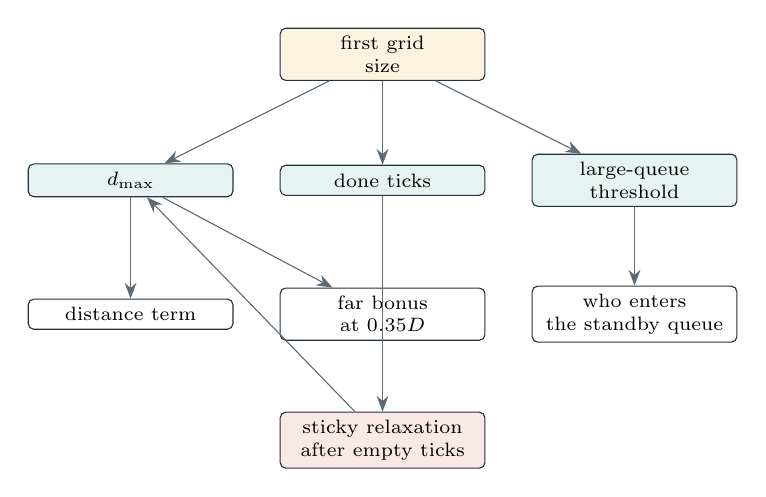
\begin{tikzpicture}[
  font=\scriptsize,
  b/.style={draw=linec, rounded corners=2pt, align=center, fill=white, inner sep=3pt,
            minimum width=26mm},
  arr/.style={-{Stealth[length=2mm]}, draw=slate}
]
  \node[b, fill=goldfaint] (map) at (0,2.2) {first grid\\size};
  \node[b, fill=tealfaint] (dmax) at (-3.2,0.6) {$d_{\max}$};
  \node[b, fill=tealfaint] (done) at (0,0.6) {done ticks};
  \node[b, fill=tealfaint] (ql) at (3.2,0.6) {large-queue\\threshold};
  \node[b] (score) at (-3.2,-1.1) {distance term};
  \node[b] (bonus) at (0,-1.1) {far bonus\\at $0.35 D$};
  \node[b] (queue) at (3.2,-1.1) {who enters\\the standby queue};
  \node[b, fill=brickfaint] (relax) at (0,-2.7) {sticky relaxation\\after empty ticks};
  \draw[arr] (map) -- (dmax);
  \draw[arr] (map) -- (done);
  \draw[arr] (map) -- (ql);
  \draw[arr] (dmax) -- (score);
  \draw[arr] (dmax) -- (bonus);
  \draw[arr] (ql) -- (queue);
  \draw[arr] (done) -- (relax);
  \draw[arr] (relax) -- (dmax);
\end{tikzpicture}%
}


\title{A Technical Account of a Failure-Managed Frontier Explorer:\\Algorithm, History, and Evidence}
\author{Author A \and Author B\\[0.4em]
\textit{Affiliation withheld}\\
\textit{Internal technical report. Companion to the concise manuscript.}}
\date{Source of record: \texttt{main} at \texttt{de8209a}.\\
Explorer file last changed in \texttt{eccbb97} (1{,}448 lines).}

\begin{document}
\maketitle

\begin{abstract}
This report is the source-level description of the frontier explorer in \texttt{Ros\_lidar\_bot}, the navigation and safety configuration that constrains it, and the commit history that produced the current policy. The explorer is not a new information-gain planner. It is a full-grid classical frontier detector whose utility is a weighted sum of cluster size, Euclidean distance, heading change, and a local free-space fraction, surrounded by a failure policy. The policy deletes unknown cells that a border-seeded flood fill cannot reach, remembers those cells as an exact set, counts Nav2 successes that leave the frontier in place, escalates repeated aborts, and keeps a geographically separated queue that a safety-stop Boolean can preempt. The report records every configured parameter and every hard-coded constant that changes a decision, the order of filters, the state of a goal, and the places where the June 2026 reference note no longer matches the code. It also records what the repository does not contain: rosbags, coverage logs, baselines, and ablations. No performance number in this document comes from a robot trial. Arithmetic examples are labelled as such. A separate assessment treats conference readiness and intellectual property. This document is the one a later experiment or a later revision should treat as the description of the implementation.
\end{abstract}

\noindent\textbf{Keywords:} frontier exploration, occupancy grid, blacklist, phantom success, Nav2, safety stop, reproducibility.

\tableofcontents
\newpage

\section{How to read this report}
The concise manuscript argues the research question in conference form. This report is the authority for behaviour. When the two disagree, this report and the source win, in that order: the source wins over both papers.

Three kinds of statement are marked as they occur.
\begin{itemize}
\item \textbf{Source.} A behaviour that follows from the current file, with a line range in \texttt{frontier\_explorer\_node.py} unless another file is named.
\item \textbf{Record.} A motivation taken from a commit message or from a comment introduced by that commit. A record is evidence of what the author wrote, not evidence that the change improved exploration.
\item \textbf{Gap.} A claim that would require a measurement the repository does not have.
\end{itemize}
Simulation worlds named in old commits (\texttt{office}, \texttt{warehouse}, \texttt{room}) are not in the \texttt{main} tree. They remain on the \texttt{Simulation} branch history. Hardware launch files are on \texttt{main}. Nothing in this study was executed on a robot or in Gazebo by the author of this report.

\section{Platform}
\subsection{What the explorer is allowed to see}
The node subscribes to \texttt{/map} (\texttt{OccupancyGrid}), \texttt{/safety\_blocked} (\texttt{Bool}), and \texttt{/manual\_blacklist} (\texttt{String}). It looks up \texttt{map}$\rightarrow$\texttt{base\_footprint}. It publishes \texttt{/frontier\_debug} (\texttt{MarkerArray}) and action goals on \texttt{navigate\_to\_pose}. It does not subscribe to \texttt{/scan}, \texttt{/cmd\_vel}, the camera, or the YOLO topics. Semantic markers cannot change a frontier score. That is a scope limit, not an oversight discovered in a comment: the subscriptions are the complete list (lines 155--161).

\begin{figure}[ht]
\centering
\FigArchitecture
\caption{Process boundary. Teal nodes are in this repository. Arrows are the topics and the action that the explorer actually uses. The camera pipeline is absent because it is absent from the node.}
\label{fig:arch}
\end{figure}

\subsection{Command path}
\texttt{config/nav2\_params.yaml} documents the Jazzy chain: regulated pure pursuit writes a navigation command, a velocity smoother follows, the collision monitor follows, and only then does \texttt{/cmd\_vel} reach the safety stop, which publishes \texttt{/cmd\_vel\_safe} for the driver. Launch comments in \texttt{launch\_robot.launch.py} still say Nav2 publishes \texttt{/cmd\_vel} directly into the safety stop. The parameter file is the wiring that \texttt{navigation\_launch.py} is given. This report follows the parameter file. The chain was not observed at runtime.

\begin{figure}[ht]
\centering
\FigCommandChain
\caption{Command path as configured, not as re-measured. PolygonSlow is enabled. PolygonStop is present and disabled. Regulated pure pursuit collision checking is off.}
\label{fig:chain}
\end{figure}

The collision polygon that is enabled is a slowdown box from $x=0.30$\,m to $0.65$\,m and $|y|\le 0.24$\,m, with \texttt{slowdown\_ratio} $0.5$. The stop polygon from $0.30$\,m to $0.40$\,m is disabled. The safety stop is therefore the hard gate. It is not the first gate: a person inside the slowdown box can already have halved the command.

\subsection{Safety stop}
\label{sec:safety}
\texttt{safety\_stop\_node.py} and the parameters in \texttt{launch\_robot.launch.py} (lines 222--236) agree. The values below are the launched values, not the defaults that would apply if the node were started alone. The defaults happen to match.

\begin{table}[ht]
\centering
\caption{Safety-stop parameters that the explorer can observe, directly or through a blocked robot.}
\label{tab:safety}
\small
\begin{tabular}{@{}llll@{}}
\toprule
Name & Value & Unit & Effect on exploration \\
\midrule
\texttt{min\_safe\_distance} & 0.35 & m & Forward block engages \\
\texttt{clear\_margin} & 0.10 & m & Release only beyond 0.45\,m \\
\texttt{ignore\_below} & 0.30 & m & Chassis returns ignored \\
\texttt{front\_opening\_deg} & 50 & deg & Total width, so $\pm 25^\circ$ \\
\texttt{rear\_opening\_deg} & 50 & deg & Reverse only; does not set the Boolean \\
\texttt{odom\_raw\_timeout\_sec} & 0.5 & s & Silence zeroes all motion and sets the Boolean \\
\bottomrule
\end{tabular}
\end{table}

\begin{figure}[ht]
\centering
\FigSafetyCone
\caption{Laser sectors. Only the forward sector, or stale \texttt{/odom\_raw}, raises \texttt{/safety\_blocked}. Yaw rate is copied through unchanged, so a spin recovery still turns the robot while translation is zero.}
\label{fig:cone}
\end{figure}

The Boolean is published from the scan callback when the forward state is recomputed, and from the 10\,Hz watchdog when odometry is stale. It is not a fixed 20\,Hz stream. The June report's ``20\,Hz'' and its $0.25$\,m, $180^\circ$ cone are the old simulation launch, not this bringup. The cone was narrowed on 26 July 2026 (\commit{91d464f}). The commit message says a $\pm 90^\circ$ cone froze the robot when a person stood beside it. That is a record of intent. There is no count of freeze events.

The explorer's own timer is 3\,s. It stores the time of the rising edge and preempts when the Boolean has stayed true for more than 3\,s at a tick (lines 290--318). The effective delay is therefore the threshold plus up to one timer period. A rear-only block never starts that clock. An odometry dropout does, and the goal is then blacklisted even though the map may be fine.

\subsection{Navigation parameters that change exploration outcomes}
These are not explorer parameters. They decide whether a goal the explorer sends is reached, aborted, or stalled.

\begin{table}[ht]
\centering
\caption{Nav2 settings that interact with the explorer. Source: \texttt{config/nav2\_params.yaml}.}
\label{tab:nav}
\small
\begin{tabular}{@{}p{5.6cm}p{2.2cm}p{6.4cm}@{}}
\toprule
Setting & Value & Interaction \\
\midrule
Planner & NavFn, A* & \texttt{allow\_unknown: true}, tolerance 0.5\,m. Goals lie in free cells, but the path may enter unknown space. \\
\texttt{xy\_goal\_tolerance} & 0.30\,m & Nav2 can succeed before the explorer's 0.45\,m bookkeeping radius. \\
\texttt{yaw\_goal\_tolerance} & 0.50\,rad & Orientation is the bearing from the robot to the goal at send time. It is not tracked afterwards. \\
Pose progress checker & 0.08\,m or 0.30\,rad within 25\,s & Rotation counts. The explorer's stall test does not. \\
\texttt{desired\_linear\_vel} & 0.35\,m/s & Kinematic lower bound only. A 5.5\,m goal takes at least $5.5/0.35\approx 16$\,s of translation, ignoring turns and the slowdown polygon. \\
\texttt{use\_rotate\_to\_heading} & true & Turn in place above 0.4\,rad, yaw rate 1.0\,rad/s. Re-enabled 20 July after a dead-odometry spin was charged to this flag. The safety stop now zeroes motion if \texttt{/odom\_raw} dies. \\
\texttt{use\_collision\_detection} & false & RPP does not stop on its own lookahead. \\
Local inflation & 0.28\,m & Footprint is a $0.50\times 0.36$\,m rectangle. \\
Global inflation & 0.35\,m & Lowered from 0.45\,m so one person does not seal a corridor. Record, not a trial. \\
\texttt{transform\_tolerance} & 1.0\,s & Several servers. Comment says map$\rightarrow$odom lagged about 0.6\,s on the Pi under DenseBoost. \\
Behaviour plugins & spin, backup, wait & No behaviour tree file is in the repository. Recovery order is Nav2's default for this plugin list. \\
\bottomrule
\end{tabular}
\end{table}

SLAM Toolbox runs in online async mode. Resolution is $0.05$\,m. Minimum laser range in the SLAM file is $0.45$\,m. The scan filter that actually edits \texttt{/scan} uses $0.30$\,m (\texttt{launch\_robot.launch.py}). Those two floors differ. The explorer never reads the scan, so the difference matters only through the map and through the safety stop, which sees the filtered scan and then ignores returns below $0.30$\,m again.

Startup order is SLAM at 5\,s, Nav2 at 8\,s, explorer at 22\,s (\texttt{autonomous\_robot.launch.py}, lines 61--65). The 22\,s delay is a fixed timer, not a wait on the action server. The server wait of 1\,s happens later, inside each goal send.

\section{Problem formulation}
\subsection{Grid and pose}
Let $M$ be the latest occupancy grid, width $W$, height $H$, resolution $\rho$, origin $(o_x,o_y)$. Cell $(i,j)$ has world centre
\begin{equation}
\big(o_x+(i+\tfrac12)\rho,\; o_y+(j+\tfrac12)\rho\big).
\label{eq:centre}
\end{equation}
The implementation classifies a cell as free only when its integer value is $0$ and unknown only when it is $-1$ (lines 960--961). Occupied cells are typically $100$ under SLAM Toolbox's trinary maps. Any other value, including a probabilistic midpoint, is neither free nor unknown: it blocks the flood fill and it is not a frontier neighbour. The report does not claim the live map is trinary. The mapper file does not set a map mode.

The pose $p=(x,y,\psi)$ is the translation and yaw of \texttt{base\_footprint} in \texttt{map}. Yaw is the standard $z$-$w$ extraction (lines 1131--1134). If the transform is missing, the tick returns. No goal is sent and the empty-tick counter is not incremented, because the increment sits after a successful pose lookup on the idle path (lines 382--408).

\subsection{Frontier}
An unknown cell is a frontier cell when at least one of its eight neighbours is free. The four roll-shifts that build that test wrap around the array, so the code then clears the entire border of the mask (lines 1022--1038). Frontier cells on the outer row and column are never detected, regardless of the later border margin.

Clusters are the 8-connected components of that set (lines 1054--1071). The representative point $g(F)$ is not the centroid. The centroid index is the rounded mean of member indices. Among free 8-neighbours of any member, $g$ is the one with smallest squared index distance to that centroid, placed at the cell centre \eqref{eq:centre} (lines 1073--1103). If no free neighbour exists, the cluster is dropped. The robot is asked to drive to known free space beside the unknown set. NavFn may still plan through unknown cells.

\subsection{Decision}
On each idle tick the policy outputs either a pose or nothing. The pose orientation is the bearing from the robot to $g$ at send time (lines 520--530). It is not updated as the robot moves. During a goal the policy may cancel, blacklist, and replace the pose. It has no terminal state. ``Exploration complete'' is a log emitted when the empty counter reaches its patience (lines 411--414). The timer continues, relaxation continues, and a later candidate is still sent.

\subsection{Research question, stated as a question}
The implementation embodies this question and does not answer it.

\begin{quote}
On a classical frontier detector feeding an unmodified Nav2 stack, do an exact-cell rejection of enclosed unknown space, a counter of successes that leave unknown cells in place, and a safety-triggered standby queue reduce repeated goals in the same map region, relative to nearest-frontier and to a gain-over-path-cost utility, without a compensating loss of coverage?
\end{quote}

Section~\ref{sec:protocol} turns the question into measurements. Section~\ref{sec:evidence} states the present answer: not known.

\section{Related work and the novelty boundary}
Nearest-frontier exploration is Yamauchi's rule \cite{yamauchi1997,yamauchi1998}. Utility exploration replaces distance with a trade of expected information against a cost \cite{gonzalez2002,makarenko2002,stachniss2005}. Holz, Basilico, Amigoni, and Behnke showed that the ranking of those strategies is environment-dependent and that the cost model can dominate the gain model \cite{holz2010}. Fast detectors avoid a full-grid scan \cite{keidar2014,quin2014}. Sampling-based detectors avoid an explicit boundary \cite{umari2017}. \texttt{explore\_lite} clusters frontiers, scores a gain against a path cost, and blacklists failures \cite{horner2016}.

Table~\ref{tab:prior} places the implementation against that set. ``Present'' means the source does it. ``Absent'' means it does not. Neither column is a quality judgment.

\begin{table}[ht]
\centering
\caption{What is and is not in the explorer, relative to standard practice.}
\label{tab:prior}
\small
\begin{tabular}{@{}p{4.2cm}p{3.4cm}p{6.6cm}@{}}
\toprule
Idea & In this source? & Note \\
\midrule
Unknown cell beside free space & Present & 8-connected. Yamauchi used the free-side boundary; the goal here is moved back onto free space. \\
Full-grid extraction each decision & Present & Not WFD, not RRT. \\
Linear utility of size, distance, heading, openness & Present & Weights are configured, not learned. \\
Path cost or information gain & Absent & Distance is Euclidean. Size stands in for gain. \\
Blacklist of failed goals & Present & Also in \texttt{explore\_lite}. Radius and timeout adapt with hits. \\
Enclosed-void removal & Present & 4-connected flood from the map border. The predicate is an exact cell set, not a disk. \\
Success that does not clear the map & Present & Counted separately from abort. Threshold 2. \\
External safety Boolean as a goal switch & Present & 3\,s, then the queue. \\
Multi-robot, semantic goals, next-best-view raycast & Absent & Camera stack is parallel and unused. \\
\bottomrule
\end{tabular}
\end{table}

The combination in the last three ``present'' rows is the only part that should be described as the authors' packaging. It is not, on the evidence in this repository, a demonstrated improvement, and it is not a licence to claim the surrounding classical method. A prior-art search is still required before any of those three rows is called new. Flood-fill of unreachable cells and goal blacklists are old. The exact-cell encoding and the phantom counter are specific; specificity is not novelty.

\section{Detection, pruning, and score}
\subsection{Enclosed unknown space}
\begin{figure}[ht]
\centering
\FigEnclosed
\caption{Schematic grid. Red cells are unknown and not 4-connected to the border through free or unknown cells. They are rewritten to occupied in a copy. Teal cells can seed a frontier. This is not a recorded map.}
\label{fig:enc}
\end{figure}

Define $C=\{cells=0\}$ and $U=\{cells=-1\}$. The fill (lines 899--930) is a 4-connected BFS on $C\cup U$, seeded from every traversable border cell. Enclosed cells are $U$ minus the reachable set. If any exist, the grid copy sets them to $100$ before frontier extraction (lines 963--976). Frontiers are then computed on that copy.

Each component with at least three cells may become a permanent zone (lines 991--1015):
\begin{itemize}
\item the centroid in world coordinates is inserted if no existing centroid lies inside a squared radius $(2 r_b)^2$, where $r_b$ is \texttt{goal\_blacklist\_radius} ($0.80$\,m, so $1.60$\,m);
\item every cell of the component, plus a one-cell Chebyshev buffer, is stored as the integer key $\big(\mathrm{round}(x/\rho),\,\mathrm{round}(y/\rho)\big)$.
\end{itemize}
Components of one or two cells are still removed from frontier extraction. They simply get no permanent entry. The SLAM map is never written. The zones accumulate for the process lifetime and are not pruned when the grid origin shifts. The comment in the source says world keys remain valid across origin shifts. That is true only while $\rho$ is constant and the rounding function is the same at insertion and at query. Both are true today. Alias is a separate problem, worked in Section~\ref{sec:examples}.

The marker for a permanent zone is a cylinder of radius $1.60$\,m (lines 1325--1342). The predicate is the cell set (lines 1231--1238). An operator looking at RViz sees a larger exclusion than the test applies.

Connectivity does not match. The fill is 4-connected. Frontier adjacency is 8-connected. A diagonal corridor of unknown cells can be classified as enclosed and, were it not rewritten, could also have been a frontier. The rewrite happens first, so the diagonal corridor disappears. Whether that is desirable in real furniture is a \textbf{gap}.

\subsection{Prune order}
Figure~\ref{fig:prune} is the order inside \texttt{\_score\_frontiers} (lines 750--793). Counters \texttt{n\_small}, \texttt{n\_no\_target}, \texttt{n\_edge}, \texttt{n\_blacklist}, and \texttt{n\_dist} are debug logs only. The openness rejection increments \texttt{n\_edge}, so the log line conflates border rejects with wedge rejects.

\begin{figure}[ht]
\centering
\FigPrune
\caption{A cluster is scored only if it passes every test. The openness floor and the border test are hard gates, not soft penalties.}
\label{fig:prune}
\end{figure}

The border gate is
\begin{equation}
m=\max\big(1,\,\mathrm{int}(d_{\mathrm{wall}}/\rho)\big),
\label{eq:margin}
\end{equation}
and the goal's cell index must lie in $[m,\,W-m)\times[m,\,H-m)$. With the launched $d_{\mathrm{wall}}=0.15$\,m and $\rho=0.05$\,m, $0.15/0.05$ is the float $2.999\ldots$, and Python \texttt{int} truncates toward zero, so $m=2$, not the $3$ written in the YAML comment and in the June report. The accepted cell nearest the border has its centre $2.5\rho=0.125$\,m from the map edge, which is inside the $0.15$\,m the parameter name suggests. The test is an index margin, not a Euclidean distance to the boundary.

Openness uses a square window of radius $3$ cells, not a disk (lines 1105--1128):
\begin{equation}
\Omega(g)=\frac{\#\{cells\ \mathrm{in}\ [-3,3]^2\ \mathrm{with\ value}\ 0\}}{\#\{cells\ \mathrm{of\ that\ window\ inside\ the\ grid}\}}.
\label{eq:open}
\end{equation}
The floor is $\Omega\ge 0.15$, hard-coded. On 13 May the previous floor of $0.25$ was removed (\commit{82dbf87}). The message says it rejected all tight frontiers in warehouse and office worlds. On 3 June a floor of $0.15$ was put back (\commit{6b7e6c2}) with a comment that it should catch only solid-furniture wedges. No rejection counts are stored for either change.

If the pass at $D=d_{\max}$ returns no goal, the same clusters are scored once more at $D=\min(2 d_{\max},\,d_{\mathrm{cap}})$ with $d_{\mathrm{cap}}=12$\,m (lines 709--718). Expansion is one step, not a loop. Both passes rebuild the queue.

\subsection{Utility}
Let $S=\max|F|$ over the clusters of this call, and let $D$ be the distance limit of this pass. For robot pose $p$ and yaw $\psi$,
\begin{align}
\sigma_{\mathrm{size}}&=|F|/S, &
\sigma_{\mathrm{dist}}&=\|g-p\|/D, \nonumber\\
\sigma_{\mathrm{head}}&=|\mathrm{wrap}(\operatorname{atan2}(g_y-y,g_x-x)-\psi)|/\pi, \nonumber\\
\sigma_{\mathrm{open}}&=\Omega(g).
\label{eq:terms}
\end{align}
\begin{equation}
J(F)= w_s\sigma_{\mathrm{size}}-w_d\sigma_{\mathrm{dist}}-w_h\sigma_{\mathrm{head}}+w_o\sigma_{\mathrm{open}}.
\label{eq:score}
\end{equation}
Launched weights are $w_s=1.8$, $w_d=1.0$, $w_h=0.5$, $w_o=0.7$. The node's \texttt{declare\_parameter} defaults differ ($1.5$, $1.0$, $0.8$, $0.4$) and apply only if the YAML file is not loaded. \texttt{autonomous\_robot.launch.py} loads the YAML.

If every survivor has $\|g-p\|>0.35D$, each distance term is replaced before $J$ is recomputed:
\begin{equation}
\sigma_{\mathrm{dist}}\leftarrow \max\big(0,\;\|g-p\|/D-\beta\big),
\quad
\beta=\min(0.40,\;0.45\,|F|/S).
\label{eq:far}
\end{equation}
The constants $0.35$, $0.40$, and $0.45$ are hard-coded (lines 816--845). A near survivor, even a poor one, suppresses the bonus for everyone. The bonus cannot create a candidate that pruning already removed.

\subsection{Queue construction}
When \texttt{collect\_all} is true, which it always is in the two call sites, survivors are sorted by $J$. The best is the return value and is not queued. From the remainder, up to $n_q=5$ points are kept if $|F|\ge n_L$ and each is at least $2.5 r_b$ from the others. At $r_b=0.80$\,m that separation is $2.0$\,m. If none qualify, the size test is skipped and any remainder may fill the five slots (lines 854--888). $n_L$ is set once, on the first map:
\begin{equation}
n_L=\max(3 s_{\min},\,15,\,\lfloor 0.0015\,WH\rfloor),
\label{eq:nl}
\end{equation}
with $s_{\min}$ the minimum cluster size at calibration time, which is the configured $3$ unless something else changed it first. Nothing else runs before the first map callback. Later relaxation of $s_{\min}$ does not recompute $n_L$.

\begin{figure}[ht]
\centering
\FigQueue
\caption{Queue geometry at the configured blacklist radius. The best cluster is withheld from the queue because the full scan returns it directly. The idle loop does not use that return value when the queue is non-empty. See Section~\ref{sec:tick}.}
\label{fig:queue}
\end{figure}

The queue stores $(g, J, |F|, \|g-p\|)$ only while sorting. The retained list stores $(g, J)$. On pop, $J$ is ignored.

\subsection{Pop score}
\label{sec:pop}
\texttt{\_pop\_queued\_frontier} (lines 463--510) discards a queue older than $20$\,s. Otherwise it pops from the front and skips a point that is blacklisted, whose $0.8$\,m neighbourhood contains no unknown cell, whose distance from the robot is outside $[d_{\min},\,d_{\mathrm{cap}}]$, or whose distance from the last blacklisted point is below $2 r_b$. The distance ceiling is the cap, $12$\,m, not $d_{\max}$. A point admitted when the search radius was $5.5$\,m can be dispatched later from $10$\,m away.

The score returned with a valid pop is not $J$. It is
\begin{equation}
J_{\mathrm{pop}}=-\,\|g-p\|/d_{\max}.
\label{eq:pop}
\end{equation}
$d_{\max}$ may already have been relaxed to $12$\,m, which changes $J_{\mathrm{pop}}$ even for the same point. The hysteresis test on the idle path (lines 423--427) is
\begin{equation}
\mathrm{send\ only\ if\ } g_{\mathrm{active}}=\varnothing \mathrm{\ or\ } J \ge J_{\mathrm{active}}+0.20.
\label{eq:hyst}
\end{equation}
It compares $J_{\mathrm{pop}}$ with a previously stored $J$ whenever the previous goal position has not been cleared. Those quantities do not share a zero or a scale. Figure~\ref{fig:scale} uses the numbers from the worked example in Section~\ref{sec:examples}. During an active goal the test is not used; preemption sends the popped goal unconditionally.

\begin{figure}[ht]
\centering
\FigScaleBug
\caption{Scale break between \eqref{eq:score} and \eqref{eq:pop}. The hysteresis margin of $0.20$ assumes the left-hand and right-hand scores are the same function.}
\label{fig:scale}
\end{figure}

\section{Execution}
\label{sec:tick}
\subsection{Timer}
\texttt{goal\_interval\_sec} ($3.0$\,s) is the period of \texttt{\_tick}. It is not stored on the object. Every timeout below is sampled on this period.

The tick has two halves. If \texttt{goal\_in\_progress} is true, the node may cancel or replace the goal and then returns. It does not select a fresh goal in the fall-through sense: after a failed attempt to pop a replacement it still returns, because the refresh-and-return at lines 359--375 is inside the in-progress branch and is reached whenever the earlier branches do not return. There is one exception of structure. The timeout branch sets \texttt{goal\_in\_progress} false and, if no replacement is sent, does not return inside that branch. Control then falls through the progress \texttt{elif} (skipped, because the \texttt{if} was taken) into the queue refresh, and then returns. The next period takes the idle half, subject to the cooldown.

If no goal is in progress, a cooldown of \texttt{goal\_cooldown\_sec} ($3.0$\,s) measured from \texttt{last\_goal\_end\_time} causes an immediate return. That return does not increment the empty counter. After cooldown, the node tries the queue first and a full scan only if the pop returns nothing (lines 396--405). This is the behaviour introduced as ``Q1 used in normal flow'' (\commit{818e294}) and extended so that a vanished frontier and a timeout also try the queue (\commit{b79ad0d}). The consequence is that a queue younger than $20$\,s suppresses a rescan. The next goal is a previous runner-up that survives revalidation, not the current best frontier.

\subsection{In-progress checks, in order}
The order is the order in the source, and it matters.

\begin{enumerate}
\item If the active point's $0.8$\,m neighbourhood contains no unknown cell, set the clean-cancel flag, cancel, and try the queue. Do not blacklist (lines 261--288). The radius $0.8$\,m is hard-coded, not $r_b$. At $\rho=0.05$\,m, $\mathrm{int}(0.8/0.05)=16$ cells.
\item If the safety Boolean has been true longer than $3$\,s and the queue yields a point, blacklist the active point, cancel, and send (lines 290--318). If the queue is empty or the pose is missing, this branch does not return. The safety clock is not cleared unless a switch happens.
\item If the goal is older than $90$\,s, blacklist, cancel, and try the queue (lines 320--336).
\item Else if \texttt{distance\_remaining} has not fallen by more than $0.12$\,m for $25$\,s, blacklist, cancel, and try the queue (lines 337--357).
\item If the queue stamp is older than $20$\,s, run a full scan solely to rebuild the queue (lines 359--374). The returned best goal is discarded. The active goal is left alone.
\end{enumerate}

\texttt{\_feedback\_cb} (lines 664--674) updates the progress clock only when the remaining distance decreases by more than \texttt{min\_progress\_delta}. An increase, which a longer replan produces, does not reset the clock and does not replace the stored remaining distance. The next decrease is measured against the old, smaller value, so a single later sample can look like a large improvement. Until that sample, the stall clock runs. Nav2's own checker can be satisfied by a rotation of $0.30$\,rad. The explorer will still declare a stall. Both windows are $25$\,s. The YAML comment says the explorer window must be strictly longer than Nav2's \texttt{movement\_time\_allowance}. The configured values are equal, and the comment also mentions $12$\,s in the same entry. The $12$\,s figure is stale.

\subsection{Goal generation}
Each send increments \texttt{\_goal\_gen} and captures it in the accept, result, and feedback callbacks (lines 539--560, introduced in \commit{badd582}). A callback whose generation is not current returns immediately. It does not clear \texttt{\_clean\_cancel}. The flag is cleared only at the bottom of a result callback that passed the generation test (line 662).

Sequence that leaves the flag set: a clean cancel sends a replacement, which increments the generation; the old result arrives and is ignored; \texttt{\_clean\_cancel} stays true until the replacement's result callback. On that later callback, a \texttt{STATUS\_CANCELLED} takes the clean-cancel log and does not blacklist. Blacklisting for a safety or timeout cancel is done before \texttt{cancel\_goal\_async}, so the stale flag changes the log, not the exclusion. A path that expected the callback itself to blacklist would be wrong. After \commit{47a164d} the callback never blacklists on cancel.

\texttt{goal\_handle} is assigned in the accept callback. A safety preemption at 3\,s can run before that assignment if acceptance is late. The source calls \texttt{self.goal\_handle.cancel\_goal\_async()} without a null test (line 311). The initial value is \texttt{None}. This is a real crash path in the source. This report has no log showing it has occurred.

\subsection{Pseudocode}
The listings follow the source, including the queue-first idle path and the pop score. They omit marker drawing.

\begin{lstlisting}[caption={Idle and in-progress tick, abridged only by marker calls.},label={lst:tick}]
every 3.0 s:
  if no map: return
  if goal in progress:
    if unknown cells gone within 0.8 m of the goal:
      clean_cancel = True
      cancel()
      in_progress = False
      if queue pop succeeds: send(pop); return
      stamp cooldown; return
    if safety blocked for > 3 s and queue pop succeeds:
      blacklist(active); cancel(); send(pop); return
    if age > 90 s:
      blacklist(active); cancel()
      if queue pop succeeds: send(pop); return
    else if no 0.12 m drop in distance_remaining for 25 s:
      blacklist(active); cancel()
      if queue pop succeeds: send(pop); return
    if queue older than 20 s: rescan()  # queue side effect only
    return
  if within 3.0 s of last goal end: return
  if no pose: return
  prune expired blacklists
  if active goal is within 0.45 m: forget its position
  (g, J) = pop queue          # J is -distance/d_max
  if g is empty: (g, J) = full scan   # J is equation (score)
  if g is empty:
    empty_ticks += 1
    relax()
    if empty_ticks >= patience: log "complete"
    return
  empty_ticks = 0
  if active position exists and J < active_J + 0.20: return
  send(g, J)
\end{lstlisting}

\begin{lstlisting}[caption={Full scan. Permanent-zone bookkeeping is inside extraction.},label={lst:scan}]
extract:
  flood 4-connected from the border through free or unknown
  mark unreached unknown as occupied in a copy
  record components of size >= 3 as permanent cell keys
  frontier cells = unknown cells with an 8-connected free neighbour
  drop the outer row and column of that mask
  return 8-connected clusters

score(clusters, D):
  for each cluster:
    reject if size < s_min, or no free target,
      or cell index within m of the border,
      or blacklisted, or distance outside [d_min, D],
      or openness < 0.15
    keep J from equation (score)
  if all kept distances > 0.35 D:
    recompute J with the far-frontier beta
  queue = up to 5 diverse large runners-up
  return the best
\end{lstlisting}

\section{Blacklists}
\subsection{Ordinary entries}
\texttt{\_blacklist\_goal} (lines 1140--1179) merges a new point into an existing key when the squared distance is at most $(1.5 r_b)^2$, i.e.\ $1.2$\,m at the launched radius. Otherwise it inserts a new key with one hit and timeout $T_0=300$\,s. On a merge the hit count increments and, if the count is now at least $2$,
\begin{equation}
T=\min\big(T_0\cdot 2^{h-1},\;2400\big)\ \mathrm{s},
\qquad
\mathrm{radius}=2 r_b.
\label{eq:timeout}
\end{equation}
The radius used at test time is $r_b$ for one hit and $2 r_b$ for any larger hit (lines 1222--1230). It does not grow with further hits. The timeout does, until the cap. The last blacklisted point is stored for the queue's $2 r_b$ exclusion.

Expiry is checked at the start of an idle tick, not during a goal (lines 1241--1253). A goal can still be in the queue, and be popped, against an entry that has logically expired, until the next idle prune. Pop checks \texttt{\_is\_blacklisted}, which does not look at time. So expiry is idle-only.

\subsection{Aborts and phantom successes}
On \texttt{STATUS\_ABORTED} the result callback blacklists and then, if the hit count stored under the exact returned position is at least $2$, forces that counter to $10$ and that timeout to $600$\,s (lines 621--644). The force uses the position Nav2 returned, not necessarily the merged key. If the merge wrote a different key, the force can miss it, while \texttt{\_blacklist\_goal} has already doubled the radius and scaled the timeout on the merged key. The log line can say ``1st time'' in that case. The exclusion is still the doubled one. This is source behaviour, not a guess about Nav2.

On \texttt{STATUS\_SUCCEEDED}, residual unknown within $0.8$\,m increments a phantom counter whose key is the nearest existing phantom key inside $1.2$\,m, or the current point (lines 581--610). At $2$, the code temporarily sets the base timeout to $600$\,s, calls \texttt{\_blacklist\_goal} on the current point (not necessarily the phantom key), restores the base timeout, and assigns hit count $10$ on the current point. If the blacklist call merged into an older key, the scaled timeout uses $600$\,s as its base, so the second hit stores $\min(600\cdot 2,\,2400)=1200$\,s, not the $600$\,s named in the log. The log always prints ``10 min''. The stored duration can be $1200$\,s. The June report's threshold of $3$ matches \commit{6b7e6c2} and not the current source.

A success that does clear the unknown cells drops the phantom count for that exact key and clears the last-cancel exclusion.

\subsection{Manual zones}
\texttt{/manual\_blacklist} accepts JSON (lines 1181--1205). \texttt{action: clear} deletes the manual list only. An add requires $x$ and $y$. The radius defaults to $r_b$ and is at least $0.1$\,m. \texttt{duration} $\le 0$ does not expire. The dashboard (\texttt{robot\_dashboard\_node.py}, lines 581--609) converts a click from \texttt{odom} into \texttt{map} with the current transform, and it clamps the radius to $[0.1,\,5.0]$\,m before publish. If the transform lookup fails, the translation used is zero and the click is treated as already in \texttt{map}.

Manual zones are tested first in \texttt{\_is\_blacklisted}. They are disks. They do not interact with hit counts.

\subsection{State machine}
\begin{figure}[ht]
\centering
\FigLifecycle
\caption{States that exist in the variables \texttt{goal\_in\_progress}, the action status, and the blacklist. There is no done state.}
\label{fig:life}
\end{figure}

\begin{figure}[ht]
\centering
\FigRecovery
\caption{Events that cancel the active goal, and whether they blacklist. Sampled on the 3\,s timer.}
\label{fig:rec}
\end{figure}

Table~\ref{tab:events} is the authoritative event list. ``Next'' is what the source attempts on that path, not what a later idle tick might do if the attempt fails.

\begin{table}[ht]
\centering
\caption{Goal events. Radius and timeout assume a first hit at the launched $r_b$ and $T_0$, and assume the merge key matches the queried point.}
\label{tab:events}
\small
\begin{tabular}{@{}p{4.3cm}p{3.3cm}p{6.6cm}@{}}
\toprule
Event & Exclusion & Next action \\
\midrule
Success, frontier cleared & None & Idle after cooldown \\
Success, unknown remains, count $=1$ & None & Idle after cooldown \\
Success, count reaches $2$ & Double radius; timeout uses a 600\,s base & Idle after cooldown \\
Abort, first stored hit & $0.80$\,m, $300$\,s & Idle; queue already not used inside the callback \\
Abort, second hit on that key & Double radius; timeout forced to $600$\,s & Same \\
Safety $>3$\,s with a queued point & Ordinary blacklist, then cancel & Send popped goal immediately \\
Stall or $90$\,s age & Ordinary blacklist, then cancel & Pop if possible, else next idle tick \\
Frontier vanished & None (clean cancel) & Pop if possible, else cooldown \\
Cancel status in the callback & None & Whatever the pre-cancel path already did \\
Goal rejected by Nav2 & None & Cooldown, clear active goal \\
\bottomrule
\end{tabular}
\end{table}

The abort row is easy to misread against the safety row. Safety and stall preempt inside the tick and can send a replacement before the result callback. The abort callback only blacklists. It does not pop. The next goal waits for cooldown and the idle path.

\section{Calibration and relaxation}
The first map callback calls \texttt{\_calibrate\_from\_map} once (lines 178--212). Let $L$ be the larger side of that grid in metres.
\begin{align}
d_{\max} &\leftarrow \max\big(d_{\max},\,\min(0.5 L,\,12)\big), \nonumber\\
N_{\mathrm{done}} &\leftarrow \max\big(N_{\mathrm{done}},\,\lfloor 2L\rfloor\big), \nonumber\\
n_L &\leftarrow \eqref{eq:nl}.
\label{eq:cal}
\end{align}
$d_{\max}$ is only raised. A first grid whose half-diagonal-side is below $5.5$\,m leaves the search radius at the YAML value. $L$ is the canvas, not the explored room and not the building. SLAM Toolbox's first published size is not fixed in the parameter file, so the numeric outcome of \eqref{eq:cal} is not determined by this repository. The formula is.

A $10$\,m canvas gives $0.5L=5.0<5.5$, so the radius stays $5.5$\,m, and $\lfloor 2L\rfloor=20$, so patience stays $20$ ticks. The examples in the YAML comment (``10\,m room $\rightarrow$ 5.0\,m range'') describe the formula's intermediate value, not the assignment, which refuses to lower the radius. A $20$\,m canvas raises the radius to $10$\,m and patience to $40$. A $400\times 400$ canvas at $0.05$\,m is $20$\,m on a side and also sets $n_L=\lfloor 0.0015\cdot 160000\rfloor=240$ cells.

\begin{figure}[ht]
\centering
\FigInteraction
\caption{The first grid writes three knobs. Relaxation can later overwrite the search radius and the minimum distance. It does not rewrite $n_L$ or the patience.}
\label{fig:ix}
\end{figure}

Relaxation runs only on ticks that found no goal (lines 214--250). It is sticky.

\begin{figure}[ht]
\centering
\FigRelax
\caption{Schedule from the launched minimum size of 3. Tick 6 is the only moment at which the search radius is set to the cap by relaxation. Tick 9 halves the minimum distance once.}
\label{fig:relax}
\end{figure}

From $s_{\min}=3$ and $d_{\min}=0.35$\,m the running values are: tick $3$, size $2$; tick $6$, size $1$ and $d_{\max}=12$\,m; tick $9$, $d_{\min}=0.175$\,m. Further ticks do not reduce the size below $1$. Patience $20$ then logs completion and does not stop the timer. Empty ticks are not the same as elapsed time. Cooldown ticks and in-progress ticks do not increment the counter. Twenty empty ticks are at least $60$\,s of idle decisions, and longer if goals and cooldowns intervene.

\section{Worked arithmetic}
\label{sec:examples}
None of these numbers was read from a robot log. They are evaluations of the formulas at the launched weights, $\rho=0.05$\,m, and $D=5.5$\,m.

\paragraph{Ordinary score.}
Cluster size $40$, largest cluster $80$, distance $2.2$\,m, heading error $\pi/2$, openness $0.60$.
\begin{align*}
\sigma_{\mathrm{size}}&=0.50, &
\sigma_{\mathrm{dist}}&=2.2/5.5=0.40, &
\sigma_{\mathrm{head}}&=0.50, &
\sigma_{\mathrm{open}}&=0.60,\\
J&=1.8(0.50)-1.0(0.40)-0.5(0.50)\\
&\quad +0.7(0.60)=0.67.
\end{align*}
The four contributions are $+0.90$, $-0.40$, $-0.25$, $+0.42$.

\begin{figure}[ht]
\centering
\FigScore
\caption{Decomposition of the ordinary-score example. Illustrative inputs.}
\label{fig:score}
\end{figure}

\paragraph{A nearer, smaller cluster.}
Size $12$, distance $0.80$\,m, heading error $0.20$\,rad, openness $0.40$:
\[
J=1.8(12/80)-0.80/5.5-0.5(0.20/\pi)+0.7(0.40)\approx 0.373.
\]
The larger cluster wins. The far bonus does not apply, because $0.80<0.35\times 5.5=1.925$.

\paragraph{Far bonus.}
Both candidates at $4.0$\,m, heading error $0.5$\,rad, openness $0.70$, largest size $80$. For size $64$, $\beta=\min(0.40,0.45\times 0.80)=0.36$. For size $8$, $\beta=0.045$. Without the bonus the utilities are approximately $1.123$ and $-0.137$. With it they are approximately $1.483$ and $-0.092$. The large cluster gains $0.36$ and the small one gains $0.045$. Order does not change in this particular pair. A pair can be constructed where it does, because the bonus scales with size. That construction would still be arithmetic, not evidence that the bonus helps exploration.

\paragraph{Pop of the ordinary candidate.}
If the same $2.2$\,m point is later popped, $J_{\mathrm{pop}}=-2.2/5.5=-0.40$, not $0.67$. The idle gate against a stored $0.67$ is $0.67+0.20=0.87$. The pop loses.

\paragraph{Border margin.}
$\mathrm{int}(0.15/0.05)=\mathrm{int}(2.999\ldots)=2$. Cells $0$ and $1$ are rejected. Cell $2$ is accepted. Its centre is $0.125$\,m from the map edge.

\paragraph{Rounding of permanent keys.}
For $\rho=0.05$ and an origin on a grid line, the key of cell column $i$ is $\mathrm{round}(i+0.5)$. Python half-to-even rounding gives the map $0\!\rightarrow\!0$, $1\!\rightarrow\!2$, $2\!\rightarrow\!2$, $3\!\rightarrow\!4$, $4\!\rightarrow\!4$. Columns $1$ and $2$ share a key. The mask is both coarser than one cell and not a simple dilation. Querying a goal at a cell centre uses the same formula, so a goal at the centre of a stored cell hits. A goal at the centre of an aliased neighbour can hit as well.

\paragraph{Timeout schedule.}
From a $300$\,s base, hit $1$ stores $300$\,s at radius $0.80$\,m; hit $2$ stores $600$\,s at $1.60$\,m; hit $3$ stores $1200$\,s; hit $4$ and after store $2400$\,s. The second-abort override then writes $600$\,s, which is shorter than a third-hit exponential timeout if that override runs late. Phantom insertion with the temporary $600$\,s base is a different sequence, as Section~8.2 describes.

\paragraph{Kinematic lower bounds.}
At $0.35$\,m/s with no rotation and no slowdown, $5.5$\,m takes $16$\,s and $12$\,m takes $34$\,s. At half speed inside PolygonSlow the $12$\,m bound is $69$\,s, still under the $90$\,s goal timeout if the whole path were slow. These are bounds on translation time. They are not travel times.

\section{Parameters}
Table~\ref{tab:yaml} is the launched configuration. Table~\ref{tab:hard} is every hard-coded constant that changes a decision, a timeout, or a stored key. Marker sizes and colours are omitted; they do not affect the robot. Table~\ref{tab:defaults} records node defaults that the launch file overrides, because a bare \texttt{ros2 run} would not reproduce the launched policy.

\begin{longtable}{@{}p{4.0cm}p{2.3cm}p{1.2cm}p{6.3cm}@{}}
\caption{Parameters loaded from \texttt{config/frontier\_explorer.yaml} by \texttt{autonomous\_robot.launch.py}.}\label{tab:yaml}\\
\toprule
Name & Value & Unit & Role \\
\midrule
\endfirsthead
\toprule
Name & Value & Unit & Role \\
\midrule
\endhead
\texttt{map\_topic} & \texttt{/map} & -- & Occupancy grid \\
\texttt{map\_frame}, \texttt{base\_frame} & \texttt{map}, \texttt{base\_footprint} & -- & TF lookup \\
\texttt{goal\_timeout\_sec} & 90 & s & Age cancel \\
\texttt{goal\_interval\_sec} & 3.0 & s & Tick period \\
\texttt{goal\_cooldown\_sec} & 3.0 & s & Idle pause after a goal ends \\
\texttt{goal\_reached\_radius} & 0.45 & m & Clears a stored goal position when no goal is in progress \\
\texttt{progress\_timeout\_sec} & 25 & s & Stall window \\
\texttt{min\_progress\_delta} & 0.12 & m & Required drop in distance remaining \\
\texttt{min\_frontier\_size} & 3 & cell & Initial cluster floor \\
\texttt{min\_goal\_distance} & 0.35 & m & Near cutoff \\
\texttt{max\_goal\_distance} & 5.5 & m & Initial search radius \\
\texttt{max\_range\_expansion\_factor} & 2.0 & -- & One-shot rescore radius factor \\
\texttt{max\_goal\_distance\_cap} & 12 & m & Ceiling for calibration, expansion, relaxation, and pops \\
\texttt{wall\_safe\_distance} & 0.15 & m & Input to \eqref{eq:margin}; effective index margin is 2 cells \\
\texttt{goal\_blacklist\_radius} & 0.80 & m & Base exclusion; also scales merge, spread, and pop separation \\
\texttt{blacklist\_timeout\_sec} & 300 & s & Base timeout $T_0$ \\
\texttt{size\_weight} & 1.8 & -- & $w_s$ \\
\texttt{distance\_weight} & 1.0 & -- & $w_d$ \\
\texttt{heading\_weight} & 0.5 & -- & $w_h$ \\
\texttt{openness\_weight} & 0.7 & -- & $w_o$ \\
\texttt{improvement\_margin} & 0.20 & score & Idle hysteresis \\
\texttt{no\_frontier\_done\_ticks} & 20 & tick & Patience before the completion log \\
\bottomrule
\end{longtable}

\begin{longtable}{@{}p{4.6cm}p{2.0cm}p{7.4cm}@{}}
\caption{Hard-coded decision constants in \texttt{frontier\_explorer\_node.py}.}\label{tab:hard}\\
\toprule
Symbol or site & Value & Effect \\
\midrule
\endfirsthead
\toprule
Symbol or site & Value & Effect \\
\midrule
\endhead
\texttt{\_PHANTOM\_THRESHOLD} & 2 arrivals & Blacklist after repeated uncleared success \\
\texttt{\_PHANTOM\_TIMEOUT} & 600\,s & Forced abort timeout; temporary phantom base \\
\texttt{\_queue\_size} & 5 & Standby length \\
\texttt{\_queue\_max\_age} & 20\,s & Discard and refresh \\
\texttt{\_SAFETY\_SWITCH\_SEC} & 3\,s & Preempt threshold, sampled on the tick \\
Vanish and phantom radius & 0.8\,m & Unknown-cell neighbourhood; not $r_b$ \\
Openness radius & 3 cells & Window is $7\times 7$ \\
Openness floor & 0.15 & Hard reject \\
Far-zone fraction & 0.35 & Bonus only if all survivors are farther \\
Far bonus & $\min(0.40,\,0.45|F|/S)$ & Subtracted inside the distance term \\
Queue separation & $2.5 r_b$ & $2.0$\,m when $r_b=0.80$ \\
Pop exclusion from last cancel & $2 r_b$ & $1.6$\,m \\
Blacklist merge & $1.5 r_b$ & $1.2$\,m \\
Repeat radius & $2 r_b$ & Applied when hits $>1$ \\
Timeout growth & $T_0 2^{h-1}$, cap 2400\,s & On merged repeats \\
Forced hit count & 10 & Second abort and phantom; radius already saturated at 2 \\
Permanent component minimum & 3 cells & Smaller voids are filled but not stored \\
Permanent buffer & 1 cell & Chebyshev \\
Permanent marker radius & $2 r_b$ & Display only \\
Relaxation period & every 3 empty ticks & Size, then range, then minimum distance \\
Size floor & 1 cell & Relaxation stops \\
Minimum-distance floor & 0.15\,m & Half of $0.35$ is $0.175$, so the floor does not bind \\
Range-relax tick & 6 & Sets $d_{\max}$ to the cap \\
Distance-relax tick & 9 & Halves $d_{\min}$ once \\
Calibration factors & $0.5 L$, $2 L$, $0.0015 WH$ & First grid only \\
Default $\rho$ before the first map & 0.05\,m & Overwritten on calibrate \\
Accept-server wait & 1.0\,s & Runs before any goal state is written. If the server is absent the tick returns and no goal is marked in progress. \\
Manual radius floor & 0.1\,m & Explorer side; dashboard also caps at 5\,m \\
\bottomrule
\end{longtable}

\begin{table}[ht]
\centering
\caption{Node defaults that differ from the YAML. Irrelevant if the launch file is used. Dangerous if it is not.}
\label{tab:defaults}
\small
\begin{tabular}{@{}lcc@{}}
\toprule
Parameter & Declare default & YAML \\
\midrule
\texttt{min\_frontier\_size} & 8 & 3 \\
\texttt{min\_goal\_distance} & 0.40\,m & 0.35\,m \\
\texttt{max\_goal\_distance} & 6.0\,m & 5.5\,m \\
\texttt{goal\_blacklist\_radius} & 0.50\,m & 0.80\,m \\
\texttt{blacklist\_timeout\_sec} & 90\,s & 300\,s \\
\texttt{size\_weight} & 1.5 & 1.8 \\
\texttt{heading\_weight} & 0.8 & 0.5 \\
\texttt{openness\_weight} & 0.4 & 0.7 \\
\texttt{improvement\_margin} & 0.25 & 0.20 \\
\texttt{goal\_cooldown\_sec} & 2.0\,s & 3.0\,s \\
\texttt{progress\_timeout\_sec} & 18\,s & 25\,s \\
\texttt{min\_progress\_delta} & 0.15\,m & 0.12\,m \\
\texttt{no\_frontier\_done\_ticks} & 4 & 20 \\
\texttt{wall\_safe\_distance} & 0.50\,m & 0.15\,m \\
\bottomrule
\end{tabular}
\end{table}

\section{Complexity}
A full scan allocates boolean masks of size $WH$ and runs two BFS passes in the worst case: the border fill, and a labelling of the enclosed set. Frontier clustering is linear in the number of frontier cells, with 8-neighbour lookups in a hash set. Scoring is linear in the number of clusters times a $7\times 7$ window. The far-bonus rescore repeats the openness window. Permanent-zone insertion writes nine keys per enclosed cell and is not repeated for keys already present, but the flood fill itself is repeated on every scan.

The idle period is 3\,s. During a goal, a scan runs when the queue is older than 20\,s. No timing measurement is in the repository. The July notes about a Raspberry Pi 5 missing controller cycles refer to SLAM scan matching on DenseBoost clouds of about 3200 returns, not to this Python loop. Whether the flood fill is negligible beside that load is a \textbf{gap}.

Memory for permanent keys grows with the enclosed area and is never released. On a long run in a building with many small voids this set can become large. There is no measurement of its size.

\section{History}
\label{sec:history}
Figure~\ref{fig:time} is the decision history. Table~\ref{tab:hist} is the same history with the behaviour that actually changed. Hardware-only commits are omitted here; the July navigation commits are included only where they change a signal the explorer reads or a fate of the goals it sends. Line counts are \texttt{wc -l} on \texttt{frontier\_explorer\_node.py} at that commit.

\begin{figure}[ht]
\centering
\FigTimeline
\caption{Commits that changed exploration behaviour or the document that claims to describe it. Dates are the commit dates.}
\label{fig:time}
\end{figure}

\begin{longtable}{@{}p{1.9cm}p{1.7cm}p{2.0cm}p{8.2cm}@{}}
\caption{Behavioural history. ``Record'' is the commit message or the comment added with it. Where that text does not state a reason, the cell says so.}\label{tab:hist}\\
\toprule
Date & Hash & Lines & What changed, and the record \\
\midrule
\endfirsthead
\toprule
Date & Hash & Lines & What changed, and the record \\
\midrule
\endhead
12 May & \commit{f493c96} & 517 & Restored after a deleted branch. Vectorised 8-connected extraction, utility, expansion, openness floor $0.25$, border $0.60$\,m, blacklist $0.50$\,m / $90$\,s, progress window $35$\,s, patience $10$. No queue, flood fill, or phantom counter. \\
13 May & \commit{82dbf87} & 514 & Removed the $0.25$ floor. Record: it rejected all tight frontiers in warehouse and office worlds. \\
13 May & \commit{48d893c} & 589 & First-map calibration and relaxation. Record is the title. No before/after numbers. \\
14 May & \commit{9a3fee8} & -- & Message: tune inflation, SLAM rate, and blacklist for hardware. YAML continues to move; the values that remain are those of 24 May. \\
24 May & \commit{76eae0d} & -- & Border $0.60\rightarrow 0.15$\,m. Progress window $35\rightarrow 25$\,s. Comment: $0.60$\,m removed every wall-adjacent frontier because the walls lay on the map boundary. \\
24 May & \commit{d81dd84} & 599 & Stuck-position handling, faster relaxation, patience $20$, cap $12$\,m, blacklist $0.80$\,m / $300$\,s. This is the last commit that edits the YAML. \\
2 Jun & \commit{3c81dd1} & -- & Cancel when the frontier is mapped during the trip. \\
2 Jun & \commit{827026d} & 766 & Queue and safety preemption. Record: ``zero standstill time'', as an intention. \\
2 Jun & \commit{14edb83} & -- & Repeat failures double the radius. Minimum distance from the stuck point. \\
3 Jun & \commit{6b7e6c2} & 890 & Phantom counter, threshold $3$, timeout $600$\,s. Openness floor returns at $0.15$. \\
3 Jun & \commit{b75e03f} & 907 & Every abort treated as a long dead zone. Superseded the same day. \\
3 Jun & \commit{f1a9bd3} & 984 & Enclosed fill and a diverse queue. \\
3 Jun & \commit{b8676df} & 1030 & Queue prefers large clusters. Far bonus. \\
3 Jun & \commit{ab82950} & 1144 & Markers. Exponential timeout. \\
3 Jun & \commit{818e294} & 1244 & Idle path uses the queue first. Permanent zones gain a long life. Markers kept visible. \\
3 Jun & \commit{276f5cb} & 1254 & First abort is an ordinary blacklist. A second abort at that area is the long exclusion. Record: costmap resize can abort a reachable goal. \\
3 Jun & \commit{29348bf} & -- & Report v2, on the simulation history. Describes threshold $3$ and a circular permanent zone. \\
10 Jun & \commit{b79ad0d} & 1291 & Threshold $3\rightarrow 2$. $n_L$ gains the $0.0015 WH$ term. Vanish and timeout paths pop the queue. \\
10 Jun & \commit{ee00c4d} & 1318 & Clean-cancel no longer blacklists. Queue refreshes during a goal. \\
10 Jun & \commit{47a164d} & 1322 & Cancel callback does not blacklist. Removes a double write. \\
10 Jun & \commit{badd582} & 1341 & Generation counter so a stale callback cannot clear the new goal. \\
10 Jun & \commit{6ed4bb4} & -- & Nearby permanent centroids merge. Record: centroid drift duplicated markers. \\
10 Jun & \commit{5bbaf0f} & 1371 & Permanent test becomes the cell set. Record: replaces the $1.6$\,m circle. \\
19 Jul & \commit{eccbb97} & 1448 & Manual zones from the dashboard. Last edit of the explorer. \\
19 Jul & \commit{e48f411}, \commit{19bbea1} & -- & Rotate-to-heading off, then on again once the safety stop halts on dead \texttt{/odom\_raw}. \\
26 Jul & \commit{91d464f}, \commit{8547161} & -- & Cone narrowed to $50^\circ$ with hysteresis. PolygonSlow enabled. Explorer source unchanged. \\
\bottomrule
\end{longtable}

Branch \texttt{home\_updated} adds a home goal after \texttt{home\_recovery\_ticks} (default $6$) and is not merged. The record of why \texttt{main} lacks it is absent. The June report's branch table, which describes \texttt{main} as a 599-line explorer without a queue, describes an older \texttt{main}. Current \texttt{main} contains the June--July policy.

\section{Where the June report is wrong}
The note \texttt{docs/frontier\_explorer\_report\_v2.md} at \commit{29348bf} (3 June 2026) is a useful diary and a bad specification of the current source. Table~\ref{tab:legacy} lists disagreements that change a technical claim. Wording differences are ignored.

\begin{table}[ht]
\centering
\caption{Legacy report against the source on \texttt{main}.}
\label{tab:legacy}
\small
\begin{tabular}{@{}p{3.3cm}p{5.4cm}p{5.5cm}@{}}
\toprule
Topic & Report v2 & Current source \\
\midrule
Phantom threshold & 3 & 2, since \commit{b79ad0d} \\
Permanent exclusion & Disk of radius $1.60$\,m & Exact buffered cells; disk is only the marker \\
Large-queue rule & $\max(3 s_{\min}, 15)$ & Also $\lfloor 0.0015 WH\rfloor$ \\
Vanish during a trip & Rescan next tick & Pop the queue first \\
Goal timeout & Rescan next tick, in the summary table & Pop the queue on that tick \\
Termination & Node stops sending & Log only \\
Safety geometry & $0.25$\,m, front $180^\circ$, rear $60^\circ$ & $0.35$\,m, both arcs $50^\circ$, hysteresis, odometry watchdog \\
Safety topic rate & 20\,Hz & On each scan, plus the 10\,Hz watchdog when odometry is dead \\
RPP collision check & Off, and described as the only laser gate & Still off, but PolygonSlow is now in front of the safety stop \\
Border margin & 3 cells & $\mathrm{int}(0.15/0.05)=2$ cells \\
Completion formula & 10\,m room $\rightarrow$ 5\,m range & Half of 10\,m is below 5.5\,m, so the radius is not lowered \\
\bottomrule
\end{tabular}
\end{table}

The report's scoring equation, the $0.15$ openness floor, the far-bonus formula, the $3$\,s safety switch, the exponential timeout, and the two-stage abort match the source at the launched parameters. Those parts can be reused. The rest should not be quoted as current behaviour.

\section{Evidence}
\label{sec:evidence}
Searches of the tree found no rosbag, no CSV of runs, and no coverage log. The word ``verified'' in July commit messages attaches to transform tolerance, a laser-yaw correction, and the safety cone. Those messages do not state a sample size, a baseline, or an exploration metric. This report does not promote them to results.

Supported now:
\begin{itemize}
\item the decision rule, the constants, and the control flow in the sections above;
\item the existence of the design reversals in Section~\ref{sec:history}, as text in commits;
\item the disagreements in Table~\ref{tab:legacy}.
\end{itemize}

Not supported:
\begin{itemize}
\item any comparison of time, path, or coverage against another explorer;
\item any ablation of the flood fill, the phantom counter, the queue, the far bonus, or relaxation;
\item the claim that standstill time fell to zero;
\item the claim that two phantom hits are better than three;
\item the claim that exploration completes.
\end{itemize}

Negative findings that \emph{are} supported, because they are properties of the source rather than of a trial: the completion log does not stop the node; the pop score is not the selection score; the border comment does not match \eqref{eq:margin}; the permanent marker is larger than the permanent predicate; the first grid can set a queue threshold that the fallback then undoes.

\section{What an evaluation has to be}
\label{sec:protocol}
\begin{figure}[ht]
\centering
\FigExperiment
\caption{Protocol. Empty of results on purpose.}
\label{fig:exp}
\end{figure}

\paragraph{Systems.}
The same robot model, the same Nav2 file, and the same SLAM file for every method. Methods: nearest frontier with the same detector and the same blacklist-free pruning; a gain-over-cost utility whose cost is Nav2 path length and whose gain is cluster size, which is the honest \texttt{explore\_lite}-style baseline using this detector; the full policy; and ablations that remove exactly one of enclosed fill, phantom counter, queue preemption, far bonus, and relaxation. A path-cost version of the full policy is a separate row, because Euclidean cost is a confound.

\paragraph{Worlds.}
The office and warehouse worlds named in \commit{82dbf87} if they can be recovered from the \texttt{Simulation} history, plus one hardware floor with a saved map and a written layout. Worlds are not on \texttt{main} today. A comparison that uses a different map for each method is not a comparison.

\paragraph{Repeats and outcomes.}
At least twenty starts per cell, with the start pose fixed across methods and the simulator seed varied. Outcomes: time and path length to 95\,\% of the reachable free space that a human labels in advance; number of goals; number of goals whose point lies within $1.2$\,m of an earlier goal; safety-preemption count; abort count; phantom count; fraction of ticks that pop the queue instead of scanning. The reachable set has to be defined without the explorer's own flood fill, or the enclosed-region ablation cannot be scored fairly. One workable definition is the free space observed by a reference run that is not part of the comparison, unioned across methods after the fact and frozen before scoring.

\paragraph{Statistics.}
Paired tests within a world, because the start is shared. Report medians and interquartile ranges, not only means. A single impressive run is not a result. Stopping rules and excluded crashes are written down before the runs.

\paragraph{Instrumentation that the code does not yet have.}
The debug line inside scoring is at debug level and is not a trial log. A later experiment needs a structured record per goal: stamp, pose, $J$ and $J_{\mathrm{pop}}$ if both exist, cluster size, reason for ending, whether the queue was used, blacklist hits, and the unknown-cell count within $0.8$\,m. Without that record the phantom counter cannot be audited after the fact.

Until this protocol is run, the correct sentence in a conference abstract is that the policy is implemented and uncompared.

\section{Threats to validity}
\label{sec:threats}
\begin{enumerate}
\item Euclidean cost favours frontiers behind walls. A gain that looks helpful may be an artefact of that cost.
\item Cluster size is not area that the lidar will see. Openness is a $7\times 7$ free fraction, not clearance along the path.
\item The 3\,s sampler delays every preemption by up to one period and defines ``25\,s'' as ``the first tick after 25\,s''.
\item One-shot calibration on the SLAM canvas makes thresholds depend on a middleware detail that this repository does not pin down.
\item Key rounding aliases permanent cells. The RViz disk hides the alias.
\item Queue-first idle selection serves stale runners-up for up to 20\,s.
\item $J_{\mathrm{pop}}$ makes the hysteresis test and the log misleading whenever a stored four-term score is still present.
\item The safety Boolean conflates a forward obstacle with a dead encoder.
\item Equal 25\,s windows on different progress definitions let the explorer blacklist a robot that Nav2 considers to be progressing, and the reverse can occur when remaining distance falls during a spin that does not change pose enough for Nav2.
\item A null \texttt{goal\_handle} during early preemption is an unhandled exception path.
\item Semantic perception is unused, so the method neither benefits from nor is confounded by the detector. It also cannot be sold as semantic exploration.
\item The author of this report did not run the stack. A defect that is invisible statically, such as a QoS mismatch on \texttt{/map}, is not ruled out. The map subscription uses the default QoS. SLAM Toolbox map publishers are often transient-local. A default volatile subscription can miss the latched map. This report flags it as a risk, not as a reproduced failure. It should be checked before any trial.
\end{enumerate}

The QoS risk is specific enough to state carefully. The subscription is created as \texttt{create\_subscription(..., 10)} (line 155), which is a depth-10 volatile reliable subscription in rclpy. If the map publisher is transient-local, late start at 22\,s can still receive data only when the publisher sends the next update. SLAM Toolbox's \texttt{map\_update\_frequency} is $2.0$\,Hz, so a later update should arrive. A truly latched and silent map would be missed. Whether that happens on this version of SLAM Toolbox was not tested here.

\section{Reproducibility}
The following reproduces the \emph{configuration}, not a measured outcome.

\begin{enumerate}
\item Revision \texttt{de8209a} of the public repository \texttt{amey1942007/Ros\_lidar\_bot}. The explorer bytes match \commit{eccbb97}.
\item ROS 2 Jazzy, the Nav2 bringup that \texttt{launch\_robot.launch.py} includes, and SLAM Toolbox's \texttt{online\_async\_launch.py}. Versions are not pinned in the repository beyond the Jazzy migration commits of 10--16 July 2026.
\item \texttt{ros2 launch Ros\_lidar\_bot autonomous\_robot.launch.py} on the robot described by the URDF and the launch file: differential drive, footprint $0.50\times 0.36$\,m in the costmap, lidar yaw $\pi$ in \texttt{lidar.xacro}, scan mode DenseBoost. Motor and lidar product names appear in comments (DDSM115, RPLidar S2E). This report does not repeat them as independently measured hardware.
\item The YAML in Table~\ref{tab:yaml} and the hard-coded constants in Table~\ref{tab:hard}. Changing either table changes the policy.
\item Worlds for the May comments are not on \texttt{main}. Recover them from the \texttt{Simulation} history if a simulation repeat is required. Do not invent a substitute and call it the same experiment.
\end{enumerate}

A second machine that runs the node without the launch file will silently take Table~\ref{tab:defaults}. Any replication protocol has to assert that the YAML was loaded, for example by reading the parameters back from the node.

Logging at INFO shows goal points, phantom counts, aborts, and the completion line. It does not show the four terms of $J$. Those are debug logs inside scoring. A replication that needs them must enable debug for this node or add the structured log in Section~\ref{sec:protocol}.

\section{Publication and intellectual property, in brief}
The conference argument is in the concise manuscript. The short version of the judgment, justified at length in the separate assessment, is as follows.

The work is not ready for IROS, ICRA, or RA-L as a results paper. The method is describable, and this report describes it. The missing piece is the comparison in Section~\ref{sec:protocol}. A workshop paper that presents the policy as an engineered response to named failure modes, with the gaps left visible, is a more honest near-term target than a claim of improved exploration.

The repository is public and licensed Apache-2.0. That is a disclosure. It is also a patent grant to users of the code, under the terms of that licence. Whether any residual claim is worth filing is a question for counsel, and it has to be asked before a conference version is posted and with the disclosure date of the May 2026 commits in hand. This report is not a patent application and not legal advice.

\section{Conclusion}
The explorer on \texttt{main} detects classical frontiers on a full grid, scores them with \eqref{eq:score}, and wraps that score in a failure policy: enclosed unknown cells are removed and stored as rounded world keys; an uncleared Nav2 success is counted and blacklisted at two; repeated aborts widen and lengthen an exclusion; a safety Boolean, a stall, and a timeout can jump to a spatially separated runner-up. Relaxation loosens size, range, and minimum distance, and then keeps them loose. The node does not stop when it says exploration is complete.

Several of those mechanisms exist because earlier thresholds made the robot refuse real frontiers or stand still. The commits say so. They do not show that the replacements explore better than nearest-frontier or \texttt{explore\_lite}. The June report describes an intermediate program and should not be cited as the specification. The specification is the source, with the line ranges and tables in this report, until the code changes.

The useful next edit is small and prior to any new heuristic: make a popped goal carry $J$ rather than \eqref{eq:pop}, make the border test a distance, stop aliasing permanent keys, and latch or delete the completion log. The useful next measurement is the protocol in Section~\ref{sec:protocol}. Either of those is more informative than another weight.

\begin{thebibliography}{99}
\bibitem{yamauchi1997} B.~Yamauchi, ``A frontier-based approach for autonomous exploration,'' in \emph{Proc.\ IEEE Int.\ Symp.\ Computational Intelligence in Robotics and Automation}, 1997, pp.~146--151.
\bibitem{yamauchi1998} B.~Yamauchi, ``Frontier-based exploration using multiple robots,'' in \emph{Proc.\ Int.\ Conf.\ Autonomous Agents}, 1998, pp.~47--53.
\bibitem{gonzalez2002} H.~H.~Gonz\'alez-Ba\~nos and J.-C.~Latombe, ``Navigation strategies for exploring indoor environments,'' \emph{Int.\ J.\ Robotics Research}, vol.~21, no.~10--11, pp.~829--848, 2002.
\bibitem{makarenko2002} A.~A.~Makarenko, S.~B.~Williams, F.~Bourgault, and H.~F.~Durrant-Whyte, ``An experiment in integrated exploration,'' in \emph{Proc.\ IEEE/RSJ IROS}, 2002.
\bibitem{stachniss2005} C.~Stachniss, G.~Grisetti, and W.~Burgard, ``Information gain-based exploration using Rao-Blackwellized particle filters,'' in \emph{Proc.\ Robotics: Science and Systems}, 2005.
\bibitem{holz2010} D.~Holz, N.~Basilico, F.~Amigoni, and S.~Behnke, ``Evaluating the efficiency of frontier-based exploration strategies,'' in \emph{Proc.\ ISR/ROBOTIK}, 2010.
\bibitem{keidar2014} M.~Keidar and G.~A.~Kaminka, ``Efficient frontier detection for robot exploration,'' \emph{Int.\ J.\ Robotics Research}, vol.~33, no.~2, pp.~215--236, 2014.
\bibitem{quin2014} P.~Quin, A.~Alempijevic, G.~Paul, and D.~Liu, ``Expanding wavefront frontier detection: an approach for efficiently detecting frontier cells,'' in \emph{Proc.\ Australasian Conf.\ Robotics and Automation}, 2014.
\bibitem{umari2017} H.~Umari and S.~Mukhopadhyay, ``Autonomous robotic exploration based on multiple rapidly-exploring randomized trees,'' in \emph{Proc.\ IEEE/RSJ IROS}, 2017.
\bibitem{horner2016} J.~H\"orner, ``Map-merging for multi-robot system,'' Bachelor's thesis, Charles University, Prague, 2016.
\bibitem{macenski2020} S.~Macenski, F.~Mart\'in, R.~White, and J.~Gin\'es Clavero, ``The Marathon 2: A navigation system,'' in \emph{Proc.\ IEEE/RSJ IROS}, 2020.
\bibitem{macenski2021} S.~Macenski and I.~Jambrecic, ``SLAM Toolbox: SLAM for the dynamic world,'' \emph{J.\ Open Source Software}, vol.~6, no.~61, art.~2783, 2021.
\bibitem{macenski2023} S.~Macenski, S.~Singh, F.~Mart\'in, and J.~Gin\'es, ``Regulated pure pursuit for robot path tracking,'' \emph{Autonomous Robots}, vol.~47, pp.~685--694, 2023.
\end{thebibliography}

\end{document}
